% Template of basic phisics experiment 基于 article template，在此基础上做修改
% 设定文章编码类型，正文字号为五号则 zihao=5，正文字号为小四则 zihao=-4
\documentclass[zihao=5, UTF8]{article}		


% 自定义宏定义
\def\N{\mathbb{N}}
\def\F{\mathbb{F}}
\def\Z{\mathbb{Z}}
\def\Q{\mathbb{Q}}
\def\R{\mathbb{R}}
\def\C{\mathbb{C}}
\def\T{\mathbb{T}}
\def\S{\mathbb{S}}
\def\A{\mathbb{A}}
\def\I{\mathscr{I}}
\def\d{\mathrm{d}}
\def\p{\partial}


% 物理实验报告所需的其它宏包
\usepackage{ulem}   % \uline 下划线支持

% 导入基本宏包
\usepackage[UTF8]{ctex}     % 设置文档为中文语言
\usepackage[colorlinks, linkcolor=blue, anchorcolor=blue, citecolor=blue, urlcolor=blue]{hyperref}  % 宏包：自动生成超链接 (此宏包与标题中的数学环境冲突)
% \usepackage{docmute}    % 宏包：子文件导入时自动去除导言区，用于主/子文件的写作方式，\include{./51单片机笔记}即可。注：启用此宏包会导致.tex文件capacity受限。
\usepackage{amsmath}    % 宏包：数学公式
\usepackage{mathrsfs}   % 宏包：提供更多数学符号
\usepackage{amssymb}    % 宏包：提供更多数学符号
\usepackage{pifont}     % 宏包：提供了特殊符号和字体
\usepackage{extarrows}  % 宏包：更多箭头符号

% 列表环境设置
\usepackage{enumitem}   % 宏包：列表环境设置
    \setlist[enumerate]{itemsep=0pt, parsep=0pt, topsep=0pt, partopsep=0pt, leftmargin=3.5em} 
    \setlist[itemize]{itemsep=0pt, parsep=0pt, topsep=0pt, partopsep=0pt, leftmargin=3.5em}
    \newlist{circledenum}{enumerate}{1} % 创建一个新的枚举环境  
    \setlist[circledenum,1]{  
        label=\protect\circled{\arabic*}, % 使用 \arabic* 来获取当前枚举计数器的值，并用 \circled 包装它  
        ref=\arabic*, % 如果需要引用列表项，这将决定引用格式（这里仍然使用数字）
        itemsep=0pt, parsep=0pt, topsep=0pt, partopsep=0pt, leftmargin=3.5em
    }  
% 文章页面 margin 设置
\usepackage[a4paper]{geometry}  % 宏包：文章页面 margin 设置
    \geometry{top=0.75in}
    \geometry{bottom=0.75in}
    \geometry{left=0.75in}
    \geometry{right=0.75in}   % 设置上下左右页边距
    \geometry{marginparwidth=1.75cm}    % 设置边注距离（注释、标记等）

% 自定义数学环境
\usepackage{amsthm} % 宏包：数学环境配置
% theorem-line 环境自定义
    \newtheoremstyle{MyLineTheoremStyle}% <name>
        {11pt}% <space above>
        {11pt}% <space below>
        {}% <body font> 使用默认正文字体
        {}% <indent amount>
        {\bfseries}% <theorem head font> 设置标题项为加粗
        {：}% <punctuation after theorem head>
        {.5em}% <space after theorem head>
        {\textbf{#1}\thmnumber{#2}\ \ (\,\textbf{#3}\,)}% 设置标题内容顺序
    \theoremstyle{MyLineTheoremStyle} % 应用自定义的定理样式
    \newtheorem{LineTheorem}{Theorem.\,}
% theorem-block 环境自定义
    \newtheoremstyle{MyBlockTheoremStyle}% <name>
        {11pt}% <space above>
        {11pt}% <space below>
        {}% <body font> 使用默认正文字体
        {}% <indent amount>
        {\bfseries}% <theorem head font> 设置标题项为加粗
        {：\\ \indent}% <punctuation after theorem head>
        {.5em}% <space after theorem head>
        {\textbf{#1}\thmnumber{#2}\ \ (\,\textbf{#3}\,)}% 设置标题内容顺序
    \theoremstyle{MyBlockTheoremStyle} % 应用自定义的定理样式
    \newtheorem{BlockTheorem}[LineTheorem]{Theorem.\,} % 使用 LineTheorem 的计数器
% definition 环境自定义
    \newtheoremstyle{MySubsubsectionStyle}% <name>
        {11pt}% <space above>
        {11pt}% <space below>
        {}% <body font> 使用默认正文字体
        {}% <indent amount>
        {\bfseries}% <theorem head font> 设置标题项为加粗
        {：\\ \indent}% <punctuation after theorem head>
        {0pt}% <space after theorem head>
        {\textbf{#3}}% 设置标题内容顺序
    \theoremstyle{MySubsubsectionStyle} % 应用自定义的定理样式
    \newtheorem{definition}{}


% 有色文本框及其设置
\usepackage[dvipsnames,svgnames]{xcolor}    %设置插入的文本框颜色
\usepackage[strict]{changepage}     % 提供一个 adjustwidth 环境
\usepackage{framed}     % 实现方框效果
    \definecolor{graybox_color}{rgb}{0.95,0.95,0.96} % 文本框颜色。修改此行中的 rgb 数值即可改变方框纹颜色，具体颜色的rgb数值可以在网站https://colordrop.io/ 中获得。（截止目前的尝试还没有成功过，感觉单位不一样）（找到喜欢的颜色，点击下方的小眼睛，找到rgb值，复制修改即可）
    \newenvironment{graybox}{%
    \def\FrameCommand{%
    \hspace{1pt}%
    {\color{gray}\small \vrule width 2pt}%
    {\color{graybox_color}\vrule width 4pt}%
    \colorbox{graybox_color}%
    }%
    \MakeFramed{\advance\hsize-\width\FrameRestore}%
    \noindent\hspace{-4.55pt}% disable indenting first paragraph
    \begin{adjustwidth}{}{7pt}%
    \vspace{2pt}\vspace{2pt}%
    }
    {%
    \vspace{2pt}\end{adjustwidth}\endMakeFramed%
    }

% 各级标题自定义设置
\usepackage{titlesec}   
    % section标题自定义设置 
    \titleformat{\section}[hang]{\normalfont\huge\bfseries\centering}{第\,\thesection\,部分}{20pt}{}
    % subsection标题自定义设置 
    \titleformat{\subsection}[hang]{\normalfont\Large\bfseries}{\,\thesubsection\,}{8pt}{}
    % subsubsection标题自定义设置
    \titleformat{\subsubsection}[hang]{\normalfont\large\bfseries}{\,\thesubsubsection\,}{6pt}{}

% 外源代码插入设置
\usepackage{matlab-prettifier}
    \lstset{
        style=Matlab-editor,  % 继承matlab代码颜色等
    }
\usepackage[most]{tcolorbox} % 引入tcolorbox包 
\usepackage{listings} % 引入listings包
    \tcbuselibrary{listings, skins, breakable}
    \lstdefinestyle{matlabstyle}{
        language=Matlab,
        basicstyle=\small,
        breakatwhitespace=false,
        breaklines=true,
        captionpos=b,
        keepspaces=true,
        numbers=left,
        numbersep=15pt,
        showspaces=false,
        showstringspaces=false,
        showtabs=false,
        tabsize=2
    }
    \newtcblisting{matlablisting}{
        arc=0pt,
        top=0pt,
        bottom=0pt,
        left=1mm,
        listing only,
        listing style=matlabstyle,
        breakable,
        colback=white   % 选一个合适的颜色
    }

% table 支持
\usepackage{booktabs}   % 宏包：三线表
\usepackage{tabularray} % 宏包：表格排版
\usepackage{longtable}  % 宏包：长表格
\usepackage{tabularx}  % 宏包：宽表格
\usepackage{multirow}  % 宏包：表格中一格显示多个项目

% figure 设置
\usepackage{graphicx}  % 支持 jpg, png, eps, pdf 图片 
\usepackage{pdfpages}  % 支持插入 pdf 图片
\usepackage{subcaption}    % 支持子图
\usepackage{svg}       % 支持 svg 图片
    \svgsetup{
        % 指向 inkscape.exe 的路径
        inkscapeexe = C:/aa_MySame/inkscape/bin/inkscape.exe, 
        % 一定程度上修复导入后图片文字溢出几何图形的问题
        inkscapelatex = false                 
    }


% 图表进阶设置
\usepackage{float}     % 图表位置浮动设置 
\usepackage{caption}    % 图注、表注
    \captionsetup[figure]{name=图}  
    \captionsetup[table]{name=表}
    \captionsetup{labelfont=bf, font=small}

% 文章默认字体设置
    \usepackage{fontspec}   % 宏包：字体设置
       \setmainfont{SimSun}    % 设置中文字体为宋体字体
      \setCJKmainfont[AutoFakeBold=3]{SimSun} % 设置加粗字体为 SimSun 族，AutoFakeBold 可以调整字体粗细^     \setmainfont{Times New Roman} % 设置英文字体为Times New Roman


% 其它设置
    % equation 公式编号设置
        \makeatletter  
        \renewcommand{\theequation}{\thesection.\arabic{equation}}  
        \makeatother
    % 脚注设置
        \renewcommand\thefootnote{\ding{\numexpr171+\value{footnote}}}
    % 参考文献引用设置
        \bibliographystyle{unsrt}   % 设置参考文献引用格式为unsrt
        \newcommand{\upcite}[1]{\textsuperscript{\cite{#1}}}     % 自定义上角标式引用
    % 文章序言设置
        \newcommand{\cnabstractname}{序言}
        \newenvironment{cnabstract}{%
            \par\Large
            \noindent\mbox{}\hfill{\bfseries \cnabstractname}\hfill\mbox{}\par
            \vskip 2.5ex
            }{\par\vskip 2.5ex}


% 页眉页脚设置
\usepackage{fancyhdr}   %宏包：页眉页脚设置
    \pagestyle{fancy}
    \fancyhf{}
    \cfoot{\thepage}
    \renewcommand\headrulewidth{1pt}
    \renewcommand\footrulewidth{0pt}
    \rhead{\bfseries 分组序号: YK04-2}    
    \chead{《基础物理实验》实验报告,\ 韩初晓,\ 2023K8009908002}
    \lhead{2024.12.12}

% 文档信息设置
%\title{这里是标题\\The Title of the Report}
%\author{丁毅\\ \footnotesize 中国科学院大学，北京 100049\\ Yi Ding \\ %\footnotesize University of Chinese Academy of Sciences, Beijing %100049, China}
%\date{\footnotesize 2024.8 -- 2025.1}

% 开始编辑文章

\begin{document}
\noindent\begin{flushright}
    \zihao{2}{分组序号: YK04-2}
\end{flushright}

\setCJKfamilyfont{boldsong}[AutoFakeBold = {2.17}]{SimSun}
\newcommand*{\boldsong}{\CJKfamily{boldsong}}


\begin{center}\large
    \noindent{\Huge\bfseries\boldsong《基础物理实验》实验报告 }
    \\\vspace{0.4cm}
    \noindent\textit{
        \textbf{\boldsong 实验名称：}\uline{\hspace{1.7cm} RLC串联电路的谐振与暂态过程\hspace{1.7cm}}\hspace{0.4cm} 
        指导教师：\uline{\hspace{1.0cm}张智恒\hspace{1.0cm}}}
    \\\vspace{0.1cm}
    \noindent\textit{
        姓名：\uline{\,\,\,韩初晓\,\,\,}\hspace{0.2cm}
        学号：\uline{\,\,\,{\upshape 2023K8009908002}\,\,\,}\hspace{0.2cm}
        专业：\uline{\,\,\,计算机科学与技术\,\,\,}\hspace{0.2cm}
        班级：\uline{\,\,\,\upshape{2306}\,\,\,}}
    \\\vspace{0.1cm}
    \noindent\textit{
        实验日期：\uline{\,\,{\upshape 2024.12.12}\,\,}\hspace{0.2cm}
        实验地点：\uline{\,\,\,教学楼{\upshape709}\,\,\,}\hspace{0.2cm}
        是否调课/补课：\uline{\hspace{0.5cm}否\hspace{0.5cm}}\hspace{0.2cm}
        成绩：\uline{\hspace{2cm}}}
\end{center}
% \vspace{-0.2cm}
\noindent\rule{\textwidth}{0.1em}   % 分割线

% 控制目录不换页
\vspace{1cm}
\setcounter{tocdepth}{2}  % 目录深度为 2（不显示 subsubsection）
\noindent\begin{minipage}{\textwidth}\centering
\tableofcontents\thispagestyle{fancy}   % 显示页码、页眉等   
\end{minipage}  
\newpage

\section{实验目的}\thispagestyle{fancy} 

\begin{enumerate}
    \item 研究 RLC 电路的谐振现象。
    \item 了解 RLC 电路的相频特性和幅频特性。
    \item 用数字存储示波器观察 RLC 串联电路的暂态过程，理解阻尼振动规律。
\end{enumerate}

\section{实验用具}

\begin{itemize}
    \item 标准电感
    \item 标准电容
    \item 100 \(\Omega\) 标准电阻
    \item 电阻箱
    \item 电感箱
    \item 电容箱
    \item 函数发生器
    \item 示波器
    \item 数字多用表
    \item 导线等
\end{itemize}

\section{实验原理}

\subsection{串联RLC电路的基本特性}

\begin{figure}[H]
    \centering
    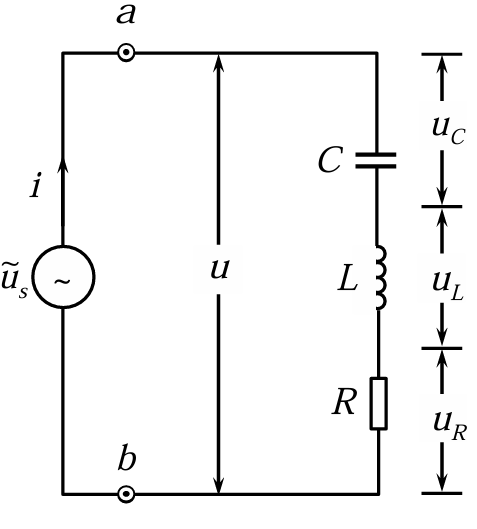
\includegraphics[width=0.5\textwidth]{./rlc_series_circuit.png}
    \caption{串联RLC电路}
    \label{fig:rlc_series_circuit}
\end{figure}


串联RLC电路由电阻\( R \)、电感\( L \)和电容\( C \)组成，其总阻抗\( Z \)可以表示为：
\[
Z = \sqrt{R^2 + \left(\omega L - \frac{1}{\omega C}\right)^2}
\]
其中，\( \omega = 2\pi f \)为角频率，\( f \)为频率。

电压\( u \)与电流\( i \)之间的相位差\( \phi \)由下式给出：
\[
\tan \phi = \frac{\omega L - \frac{1}{\omega C}}{R}
\]
因此，相位差为：
\[
\phi = \arctan\left(\frac{\omega L - \frac{1}{\omega C}}{R}\right)
\]

电流\( i \)与电压\( u \)的关系为：
\[
i = \frac{u}{Z} = \frac{u}{\sqrt{R^2 + \left(\omega L - \frac{1}{\omega C}\right)^2}}
\]

\subsection{频率特性分析}

\subsubsection{阻抗随频率变化}

随着频率\( f \)的变化，阻抗\( Z \)呈现以下特性：
\[
Z = R \quad \text{当} \quad \omega L = \frac{1}{\omega C}
\]
即当：
\[
\omega_0 = \frac{1}{\sqrt{LC}} \quad \text{或} \quad f_0 = \frac{1}{2\pi\sqrt{LC}}
\]
时，电路达到谐振状态，此时阻抗最小，为纯电阻性：
\[
Z_{\text{谐振}} = R
\]

\subsubsection{相位差随频率变化}

相位差\( \phi \)的变化特性为：
\begin{itemize}
    \item 当\( f < f_0 \)时，\( \phi > 0 \)，电路呈电容性，电流相位超前于电压。
    \item 当\( f > f_0 \)时，\( \phi < 0 \)，电路呈电感性，电流相位落后于电压。
    \item 当\( f = f_0 \)时，\( \phi = 0 \)，电压与电流同相，电路呈纯电阻性。
\end{itemize}

\subsubsection{幅频特性}

在总电压\( u \)保持不变的条件下，电流随频率的变化曲线称为幅频特性曲线。在谐振频率\( f_0 \)处，电流达到最大值：
\[
i_{\text{最大}} = \frac{u}{R}
\]

\subsection{品质因数 \( Q \) }

品质因数\( Q \)定义为：
\[
  Q = \frac{\omega_0 L}{R} = \frac{1}{\omega_0 R C} = \frac{u_L}{u} = \frac{u_C}{u}
\]
它反映了电路的储能和耗能特性：
\begin{itemize}
    \item \( Q \)值越大，电路的储能效率越高，耗能越小。
    \item 在谐振时，电感和电容上的电压均为总电压的\( Q \)倍，表现为电压谐振。
    \item \( Q \)值决定了电路的频率选择性，\( Q \)值越大，带宽越窄，频率选择性越好：
    \[
    \Delta f = \frac{f_0}{Q}
    \]
\end{itemize}

\subsection{串联谐振现象}

当电路达到谐振频率\( f_0 \)时，电感\( L \)和电容\( C \)的反应相互抵消，电路表现为纯电阻性，阻抗达到最小值\( Z = R \)，电流达到最大值\( i = \frac{u}{R} \)。此状态称为串联谐振，具有以下特点：
\begin{itemize}
    \item 电压与电流同相，\( \phi = 0 \)。
    \item 阻抗最小，电流最大。
    \item 电路表现为纯电阻性质。
\end{itemize}

\subsection{并联RLC电路的基本特性}

\begin{figure}[H]
    \centering
    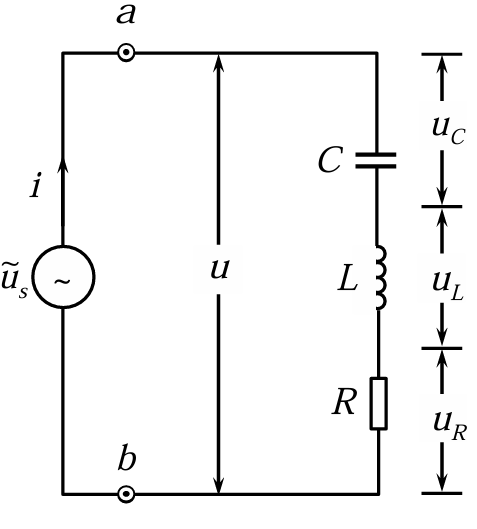
\includegraphics[width=0.5\textwidth]{./rlc_parallel_circuit.png}
    \caption{并联RLC电路}
    \label{fig:rlc_parallel_circuit}
\end{figure}

RLC并联电路由电阻\( R \)、电感\( L \)和电容\( C \)并联组成。其总阻抗\( |Z_p| \)、电压\( u \)与电流\( i \)之间的相位差\( \varphi \)关系如下：

\begin{equation}
|Z_p| = \sqrt{\frac{R^2 + (\omega L)^2}{(1 - \omega^2 LC)^2 + (\omega CR)^2}}
\end{equation}

\begin{equation}
\varphi = \arctan \left( \frac{\omega L - \omega C (R^2 + (\omega L)^2)}{R} \right)
\end{equation}

\begin{equation}
  u = i |Z_p| = \frac{u_{R'}}{R'} |Z_p|
\end{equation}

\subsection{并联谐振条件}

当相位差\( \varphi = 0 \)时，电流与电压同相，电路呈纯电阻性，发生谐振。由相位差公式可得并联谐振的角频率\( \omega_p \)（或并联谐振频率\( f_p \)）为：

\begin{equation}
\omega_p = \sqrt{\frac{1}{LC} - \left(\frac{R}{L}\right)^2} \approx \omega_0 \quad \text{当} \quad Q \gg 1
\end{equation}

\begin{equation}
f_p = \frac{\omega_p}{2\pi} \approx \frac{1}{2\pi\sqrt{LC}} = f_0
\end{equation}

其中，谐振角频率\( \omega_0 = \frac{1}{\sqrt{LC}} \)，品质因数\( Q \)定义为：

\begin{equation}
Q = \frac{\omega_0 L}{R} = \frac{\sqrt{L/C}}{R}
\end{equation}

\subsection{频率特性分析}

\subsubsection{阻抗随频率变化}

并联RLC电路的阻抗\( |Z_p| \)随频率\( f \)变化。在谐振频率\( f_p \)处，总阻抗达到最大值，电流达到最小值；当频率偏离\( f_p \)时，阻抗减小，电流增大。

\subsubsection{相位差随频率变化}

\begin{itemize}
    \item 当\( f < f_p \)时，\( \varphi < 0 \)，电流相位落后于电压，电路呈电感性。
    \item 当\( f > f_p \)时，\( \varphi > 0 \)，电流相位超前于电压，电路呈电容性。
    \item 当\( f = f_p \)时，\( \varphi = 0 \)，电压与电流同相，电路呈纯电阻性。
\end{itemize}

\subsubsection{幅频特性}

在总电流\( i \)保持不变的条件下，电压\( u \)随频率\( f \)变化。在谐振频率\( f_p \)处，电压达到最大值。

\subsection{品质因数\( Q \) }

品质因数\( Q \)反映了电路的储能与耗能特性，其定义为：

\begin{equation}
Q = \frac{\omega_0 L}{R} = \frac{1}{\omega_0 R C}
\end{equation}

\begin{equation}
\Delta f = \frac{f_p}{Q}
\end{equation}

其中，\( \Delta f \)为通频带宽度，\( Q \)值越大，带宽越窄，频率选择性越好。

\subsection{并联谐振现象}

当电路达到谐振频率\( f_p \)时，电感\( L \)和电容\( C \)的反应相互抵消，电路表现为纯电阻性，阻抗达到最大值，电流达到最小值。此状态称为并联谐振，具有以下特点：
\begin{itemize}
    \item 电压与电流同相，\( \varphi = 0 \)。
    \item 阻抗最大，电流最小。
    \item 电路表现为纯电阻性质。
\end{itemize}

在谐振时，电流在并联支路中的电感和电容上的电流分别为总电流的\( Q \)倍，称为电流谐振。

\subsection{RLC电路的暂态过程}

RLC电路由电阻\( R \)、电感\( L \)和电容\( C \)组成。在放电过程中，开关首先使电容充电至电压\( E \)，然后切换到放电位置，使电容在闭合电路中放电。电路方程为：

\[
L \frac{di}{dt} + Ri + u_C = 0
\]

将\( i = C \frac{du_C}{dt} \)代入，得到：

\[
LC \frac{d^2u_C}{dt^2} + RC \frac{du_C}{dt} + u_C = 0
\]

根据初始条件\( t = 0 \)、\( u_C = E \)、\( \frac{du_C}{dt} = 0 \)，方程的解分为三种情况：

\begin{enumerate}
    \item 当\( R^2 < 4L/C \)时，属于欠阻尼状态。引入阻尼系数\( \zeta = \frac{R}{2} \sqrt{\frac{C}{L}} \)，此时\( \zeta < 1 \)。电容电压的解为：

    \[
    u_C = \sqrt{\frac{4L}{4L - R^2C}} \, E \, e^{-t/\tau} \cos(\omega t + \varphi)
    \]

    其中，时间常量为：

    \[
    \tau = \frac{2L}{R}
    \]

    衰减振动的角频率为：

    \[
    \omega = \frac{1}{\sqrt{LC}} \sqrt{1 - \frac{R^2C}{4L}}
    \]

    此时，\( u_C \) 随时间呈指数衰减的振动，衰减速度由\( \tau \)决定，\( \tau \) 越小，衰减越快。

    \item 当\( R^2 > 4L/C \)时，属于过阻尼状态。电容电压的解为：

    \[
    u_C = \sqrt{\frac{4L}{R^2C - 4L}} \, E \, e^{-\alpha t} \sinh(\beta t + \varphi)
    \]

    其中：

    \[
    \alpha = \frac{R}{2L}, \quad \beta = \sqrt{\frac{R^2C}{4L} - 1}
    \]

    在过阻尼状态下，\( u_C \) 随时间呈指数衰减但不振荡。

    \item 当\( R^2 = 4L/C \)时，属于临界阻尼状态。电容电压的解为：

    \[
    u_C = E \left(1 + \frac{t}{\tau}\right) e^{-t/\tau}
    \]

    其中\( \tau = \frac{2L}{R} \)。这是过阻尼与欠阻尼的分界点，电压迅速达到平衡而不产生振荡。
\end{enumerate}

对于充电过程，开关切换使电源\( E \)对电容充电，电路方程变为：

\[
LC \frac{d^2u_C}{dt^2} + RC \frac{du_C}{dt} + u_C = E
\]

初始条件为\( t = 0 \)时，\( u_C = 0 \)、\( \frac{du_C}{dt} = 0 \)。其解与放电过程类似，仅最终趋向的平衡状态不同：

\begin{enumerate}
    \item 当\( R^2 < \frac{4L}{C} \)时：

    \[
    u_C = E \left[1 - \sqrt{\frac{4L}{4L - R^2C}} \, e^{-t/\tau} \cos(\omega t + \varphi)\right]
    \]

    \item 当\( R^2 > \frac{4L}{C} \)时：

    \[
    u_C = E \left[1 - \sqrt{\frac{4L}{R^2C - 4L}} \, e^{-\alpha t} \sinh(\beta t + \varphi)\right]
    \]

    \item 当\( R^2 = \frac{4L}{C} \)时：

    \[
    u_C = E \left[1 - \left(1 + \frac{t}{\tau}\right) e^{-t/\tau}\right]
    \]
\end{enumerate}

可见，充电过程和放电过程在形式上十分相似，区别在于最终趋向的平衡状态不同。


\section{实验内容}

\subsection{测RLC串联电路的相频特性和幅频特性曲线}
测量电路如图 \ref{fig:rlc_series_circuit} 所示。取 \( L = 0.1 \, \text{H} \)，\( C = 0.05 \, \mu\text{F} \)，\( R = 100 \, \Omega \)，用示波器CH1、CH2通道分别观测RLC串联电路的总电压 \( u \) 和电阻两端电压 \( u_R \)。注意两个通道的输入线的地端在 \( b \) 点共地。注意限制总电压峰峰值不超过 3.0 V（或有效值不超过 1.0 V），防止串联谐振时产生有危险的高电压。

\begin{enumerate}
  \item 调谐振，改变函数发生器的输出频率，找到谐振频率 \( f_0 \)。在谐振时，用数字多用表测量 \( u \)、\( u_L \)、\( u_C \)。利用公式$Q = \frac{u_L}{u} = \frac{u_C}{u}$计算 Q 值。
  \item 测相频特性曲线和幅频特性曲线：在总电压峰峰值 \( u_{\text{pp}} = 2.0 \, \text{V} \) 保持不变的条件下，用示波器（在双踪显示下）测出电压、电流间相位差 \( \varphi \)，以及相应的 \( u_R \)。信号频率在大约 \( 1.50 \, \text{kHz} \sim 3.30 \, \text{kHz} \) 范围内，选择相位差约 \( 0^\circ \)、\( \pm 15^\circ \)、\( \pm 30^\circ \)、\( \pm 45^\circ \)、\( \pm 60^\circ \)、\( \pm 72^\circ \)、\( \pm 80^\circ \) 所对应的频率进行测量。参考频率（单位 kHz）： 1.88、2.00、2.08、2.15、2.19、2.22、2.24、2.25、2.26、2.275、2.30、2.36、2.43、2.62、3.18。作 RLC 串联电路的 \( \varphi - f \) 曲线和 \( i - f \) 曲线。利用公式$Q = \frac{f_0}{\delta f}$估算出 Q 值。
\end{enumerate}

测量相位差的两种方法：
\begin{enumerate}
    \item （a）利用示波器左侧 MENU 按键，右侧面板上的“Measure”按键和相应的按键选取“相位 1\(\rightarrow\)2”来测量相位差。打开显示屏右侧“统计功能”，读取相位差的平均值“Avg”即可。注意：等待一会（大于 10 秒），让平均值稳定后再读数。当改变信号频率或幅度后，要先关闭“统计功能”，再打开，然后读取数据。
    \item （b）利用光标（示波器面板上“Cursor”按键）功能来读取同相位点时间间隔 \( \Delta t \)（对应示波器上显示 \( \Delta x \)）。然后利用关系式：
    \[
    \varphi = \frac{\Delta t}{T} \times 360^\circ = \Delta t \times f \times 360^\circ
    \]
    可计算出相位差。
\end{enumerate}

当改变频率而不改变函数发生器的输出电压时，外电路总电压会变小，尤其在谐振频率附近。这是由于函数发生器有 50 \(\Omega\) 内阻，而外部阻抗在谐振点附近时会明显减小。可通过适当增大函数发生器输出电压来保持总电压 \( u_{\text{pp}} = 2.0 \, \text{V} \)。

用示波器读取电压时，可读取“幅度值”或者“顶端值”，不要读取“峰峰值”，因为“峰峰值”包含了高频噪音的成分，系统误差大。

\subsection{测RLC并联电路的相频特性和幅频特性曲线}
测量电路如图 \ref{fig:rlc_parallel_circuit} 所示，取 \( L = 0.1 \, \text{H} \)，\( C = 0.05 \, \mu\text{F} \)，\( R' = 5 \, \text{k}\Omega \)（电阻 \( R' \) 是为监测总电流 \( i \) 而串入的）。为观测电感与电容并联部分的电压和相位，用CH1测量总电压，用CH2测量 \( R' \) 两端电压（注意共地点在 \( b \) 点），两通道测量电压值相减 \( \text{CH1} - \text{CH2} \) 就是并联部分的电压 \( u \)。可通过示波器面板上的“MATH”键实现两通道波形相减。

\begin{enumerate}
    \item 调谐振。改变函数发生器的输出频率，观测并联部分的电压 \( u \)（CH1-CH2）与总电流（CH2）的幅度和相位的变化。找到谐振频率 \( f_p \)。
    \item 测相频特性曲线和幅频特性曲线：固定总电压 \( u_{\text{pp}} = 2.0 \, \text{V} \) 保持不变，测量并联部分电压 \( u \)（CH1-CH2）与总电流（CH2）的相位差以及二者的幅度值。可用光标（Cursor）功能读取电压值。频率范围大约在 \( 1.70 \, \text{kHz} \sim 2.80 \, \text{kHz} \)。参考频率（单位 kHz）： 2.05、2.15、2.20、2.231、2.24、2.247、2.25、2.253、2.256、2.265、2.275、2.32、2.40、2.60。作 RLC 并联电路的 \( \varphi - f \) 曲线和 \( u - f \)、\( i - f \) 曲线。
\end{enumerate}

\subsection{观测RLC串联电路的暂态过程}

\begin{figure}[H]
    \centering
    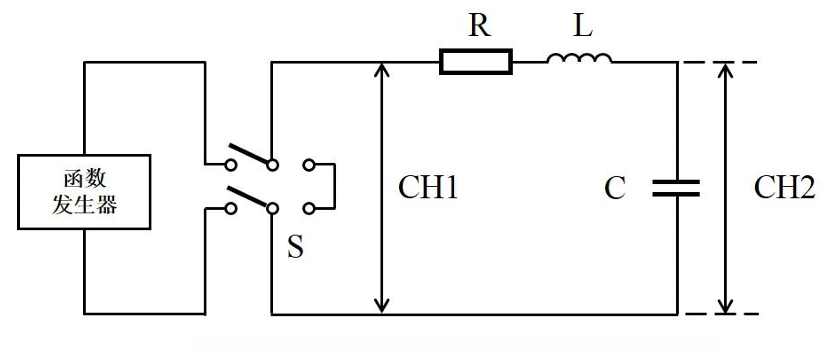
\includegraphics[width=0.5\textwidth]{./rlc_transient_process_experimental_circuit.png}
    \caption{RLC串联电路的暂态过程实验电路}
    \label{fig:rlc_transient_process_experimental_circuit}
\end{figure}

实验电路如图 \ref{fig:rlc_transient_process_experimental_circuit} 所示。由函数发生器产生方波。为便于观察，要求将方波的低电平调整与示波器的扫描基线一致。由低电平到高电平相当于充电，由高电平到低电平相当于放电。函数发生器各参数可设为：频率 50 Hz，电压峰峰值 \( u_{\text{pp}} = 2.0 \, \text{V} \)，偏移 1 V。示波器 CH1 通道用来测量总电压，CH2 用来测量电容两端电压 \( u_C \)，注意两个通道必须共地。实验中 \( L = 0.1 \, \text{H} \)，\( C = 0.2 \, \mu\text{F} \)。

\begin{enumerate}
    \item \( R = 0 \, \Omega \)，测量 \( u_C \) 波形。
    \item 调节 \( R \) 测得临界电阻 \( R_C \)，并与理论值比较。
    \item 记录 \( R = 2 \, \text{k}\Omega \)，\( 20 \, \text{k}\Omega \) 的 \( u_C \) 波形。函数发生器频率可分别选为 250 Hz（\( R = 2 \, \text{k}\Omega \)），和 20 Hz（\( R = 20 \, \text{k}\Omega \)）。
\end{enumerate}


\section{数据整理与计算}

\subsection{RLC串联电路的相频特性和幅频特性曲线}

根据公式 \( Q = \frac{\omega_0 L}{R} = 14.16 \) 计算出 Q 值。

串联电路谐振频率$f_0=2.2551kHz$，$U_L=5.62V$，$U_c=5.58V$，$U=0.466V$，$Q_L=\frac{u_L}{u} = 12.060$，$Q_C = \frac{u_C}{u} = 11.974$理论计算值为14.16，相对误差14.83\%
\begin{table}[H]
  \centering
	\begin{tabular}{|l|l|l|l|l|}
		\hline
		f/KHz & U(Vpp/V) & （CH1-CH2） & UR(Vamp) & I/mA   \\ \hline
		1.88  & 2.00     & -83.37    & 0.313    & 3.13  \\ \hline
		2     & 2.00     & -67.56    & 0.500    & 5.00  \\ \hline
		2.08  & 2.00     & -60.72    & 0.749     & 7.49  \\ \hline
		2.15  & 2.00     & -44.70    & 1.02    & 10.2  \\ \hline
		2.19  & 2.00     & -28.72    & 1.23    & 12.3  \\ \hline
		2.22  & 2.00     & -17.40     & 1.45     & 14.5 \\ \hline
		2.240 & 2.00     & -6.035    & 1.46    & 14.6  \\ \hline
		2.25  & 2.00     & -1.572      & 1.52    & 15.2 \\ \hline
		2.26  & 2.00     & 7.186     & 1.45    & 14.5  \\ \hline
		2.275 & 2.00     & 13.85     & 1.47    & 14.7 \\ \hline
		2.30  & 2.00     & 30.75     & 1.30    & 13.0 \\ \hline
		2.36  & 2.00     & 47.42     & 0.947    & 9.47  \\ \hline
		2.43  & 2.00     & 61.43     & 0.779    & 7.79  \\ \hline
		2.62  & 2.00     & 70.41     & 0.357    & 3.57  \\ \hline
		3.18  & 2.00     & 77.58     & 0.192    & 1.92  \\ \hline
	\end{tabular}
\end{table}

根据以上表格，绘制 \( \varphi - f \) 曲线和 \( i - f \) 曲线。

\begin{figure}[H]
    \centering
    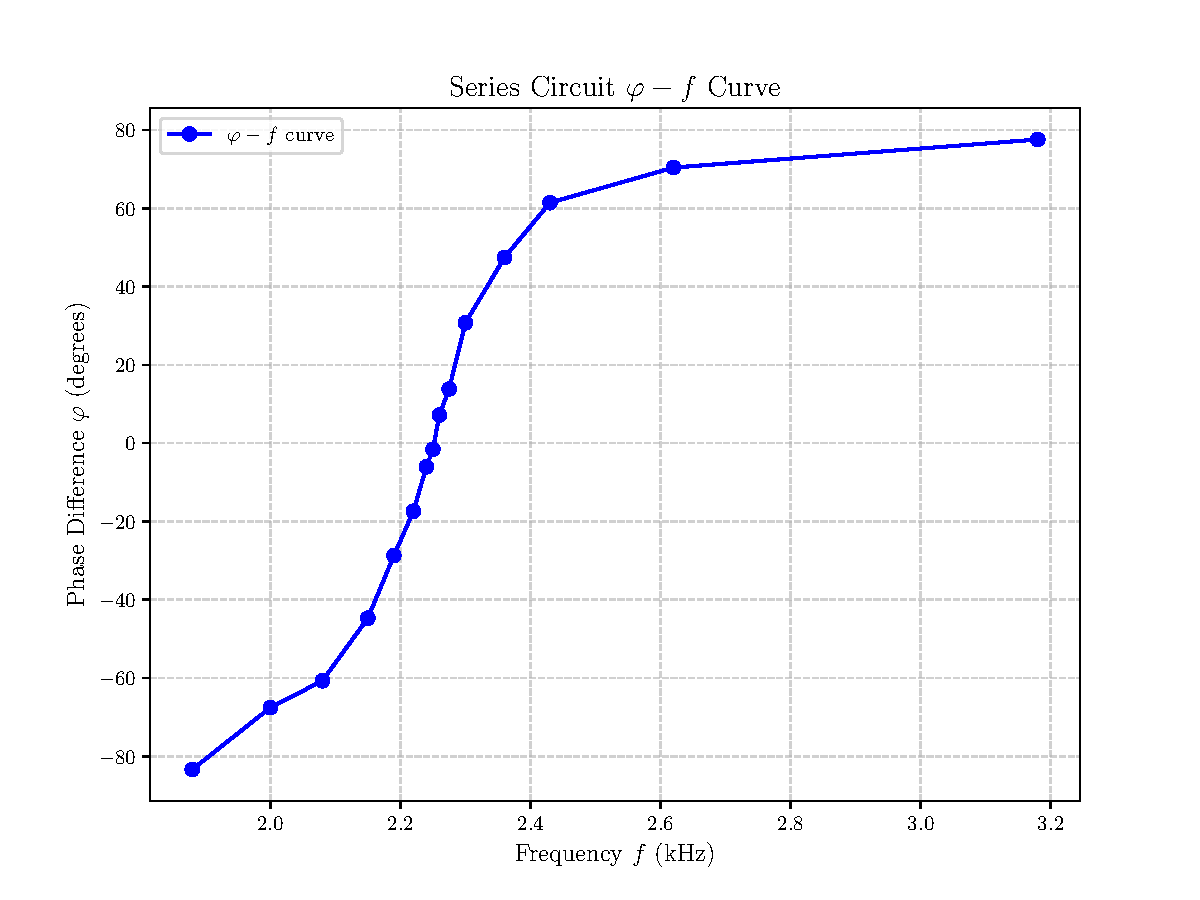
\includegraphics[width=0.8\textwidth]{./series_circuit_phi_f.pdf}
    \caption{RLC串联电路$\varphi - f$曲线}
    \label{fig:series_circuit_phi_f}
\end{figure}

观察图 \ref{fig:series_circuit_phi_f} 所示曲线可知，随着频率的变化，相位差由负变正，且相位差在谐振频率附近变化较大，而在接近 $\pm $ 90$^\circ$ 时，相位差变化较小，接近于平行于 x 轴的直线。在误差范围内与理论计算所得的图像一致。

\begin{figure}[H]
    \centering
    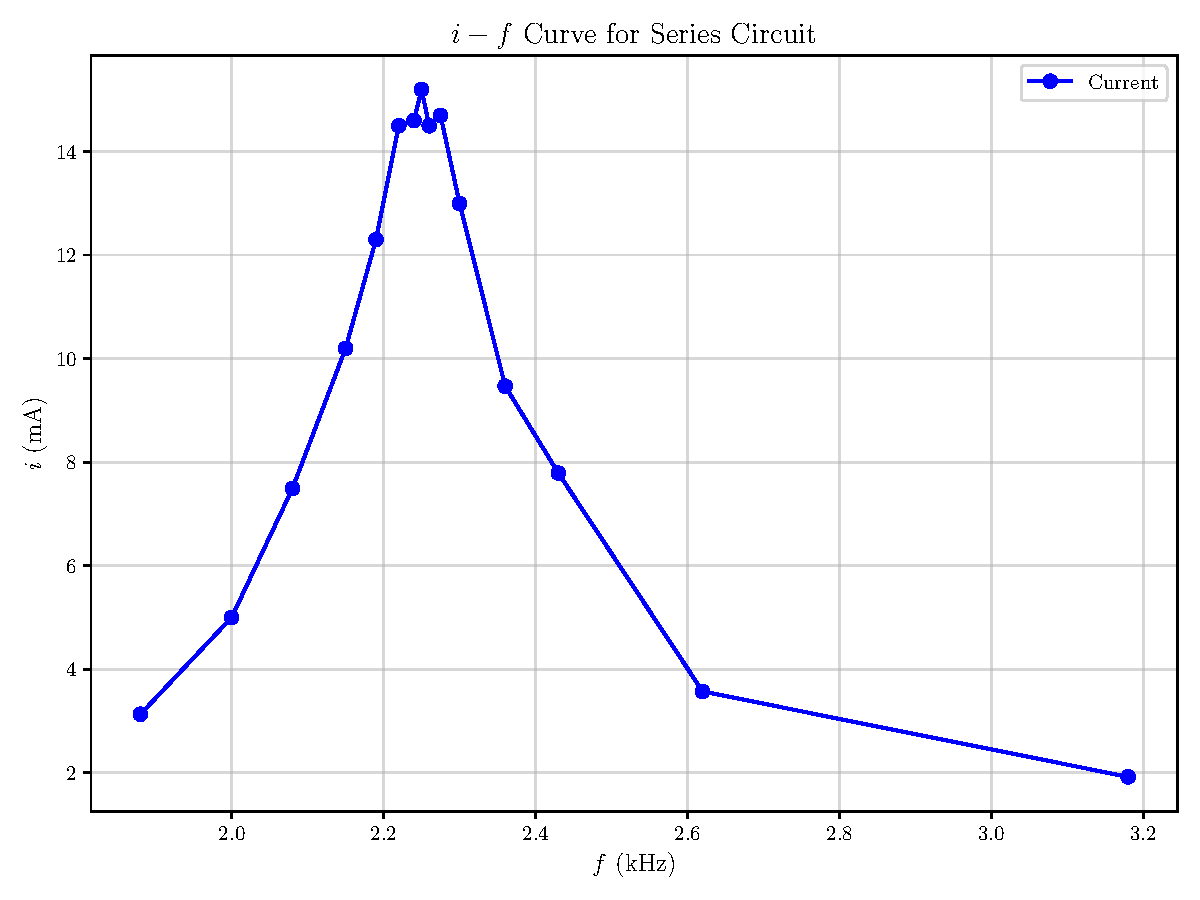
\includegraphics[width=0.8\textwidth]{./series_circuit_i_f.pdf}
    \caption{RLC串联电路$i - f$曲线}
    \label{fig:series_circuit_i_f}
\end{figure}

观察图 \ref{fig:series_circuit_i_f} 所示曲线可知，当 $f = 2.25 $ kHz 时，电流达到最大值，即 $i = 15.2$ mA。此时， $ \frac{I_{\text{max}}}{\sqrt{2}} = 10.75$ mA，在图中对应的频率约为 2.17kHz 和 2.34kHz，即带宽约为 0.17kHz。因此可求得品质因数为 $Q = \frac{f_0}{\Delta f} = 13.24$。和理论值$Q = 14.16$相比，相对误差为 6.48\%，可见测量结果比较准确。

\subsection{RLC并联电路的相频特性和幅频特性曲线}

在数据表中，根据公式$\varphi=\frac{\Delta t}{T}\times360^\circ=f\Delta t\times360^\circ$计算出相位差。

\begin{table}[H]
  \centering
	\begin{tabular}{|c|c|c|c|c|c|c|}
		\hline
    $f$/KHz & U(Vpp/V) & $\Delta t/us$ & $\varphi / ^\circ$ & （CH1-CH2） & $U_{R'}(Vamp)$/mV & $I/\mu$A  \\ \hline
		2.050 & 2.00     & 116.0              & 85.608              & 1.23      & 898      & 179.6 \\ \hline
		2.150 & 2.00     & 106.0              & 82.044              & 1.45      & 561      & 112.2 \\ \hline
		2.200 & 2.00     & 90.00              & 71.280              & 1.50      & 299      & 59.8  \\ \hline
		2.231 & 2.00     & 58.00              & 46.583              & 1.54      & 152      & 30.4  \\ \hline
		2.240 & 2.00     & 36.00              & 29.030              & 1.54      & 199      & 39.8  \\ \hline
		2.247 & 2.00     & 12.00              & 9.7070              & 1.50      & 106      & 21.2  \\ \hline
		2.250 & 2.00     & 0.000              & 0.0000              & 1.52      & 104      & 20.8  \\ \hline
		2.253 & 2.00     & -12.00             & -9.7330             & 1.51      & 105      & 21    \\ \hline
		2.256 & 2.00     & -22.00             & -17.868             & 1.54      & 110      & 22    \\ \hline
		2.265 & 2.00     & -48.00             & -39.139             & 1.49      & 142      & 28.4  \\ \hline
		2.275 & 2.00     & -66.00             & -54.054             & 1.54      & 179      & 35.8  \\ \hline
		2.320 & 2.00     & -94.00             & -78.509             & 1.45      & 381      & 76.2  \\ \hline
		2.400 & 2.00     & -98.00             & -84.672             & 1.30      & 766      & 153.2 \\ \hline
		2.600 & 2.00     & -88.00             & -82.368             & 0.915     & 1410     & 282   \\ \hline
	\end{tabular}
\end{table}

根据以上表格，绘制 \( \varphi - f \) 曲线 \( u - f\) 曲线和 \( i - f \) 曲线。

\begin{figure}[H]
    \centering
    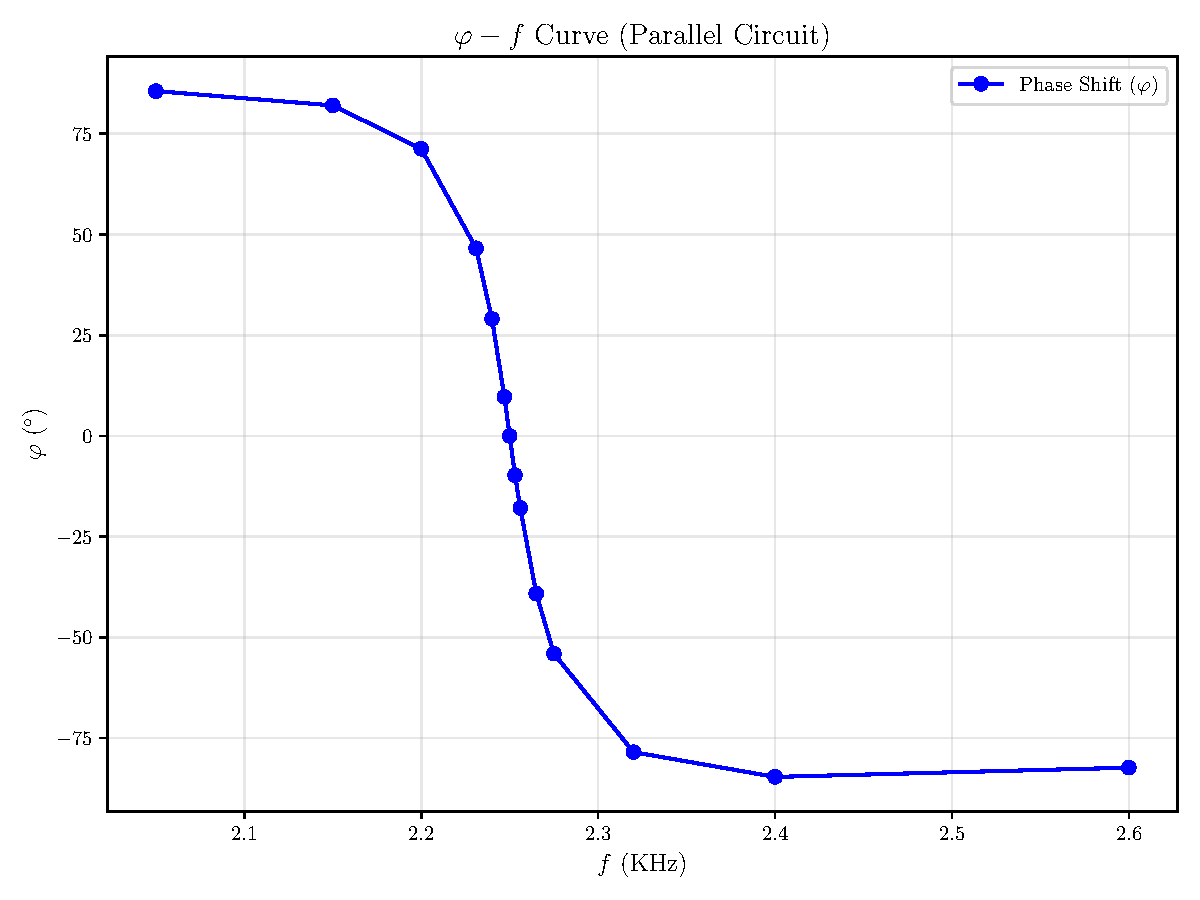
\includegraphics[width=0.8\textwidth]{./parallel_circuit_phi_f.pdf}
    \caption{RLC并联电路$\varphi - f$曲线}
    \label{fig:parallel_circuit_phi_f}
\end{figure}

\begin{figure}[H]
    \centering
    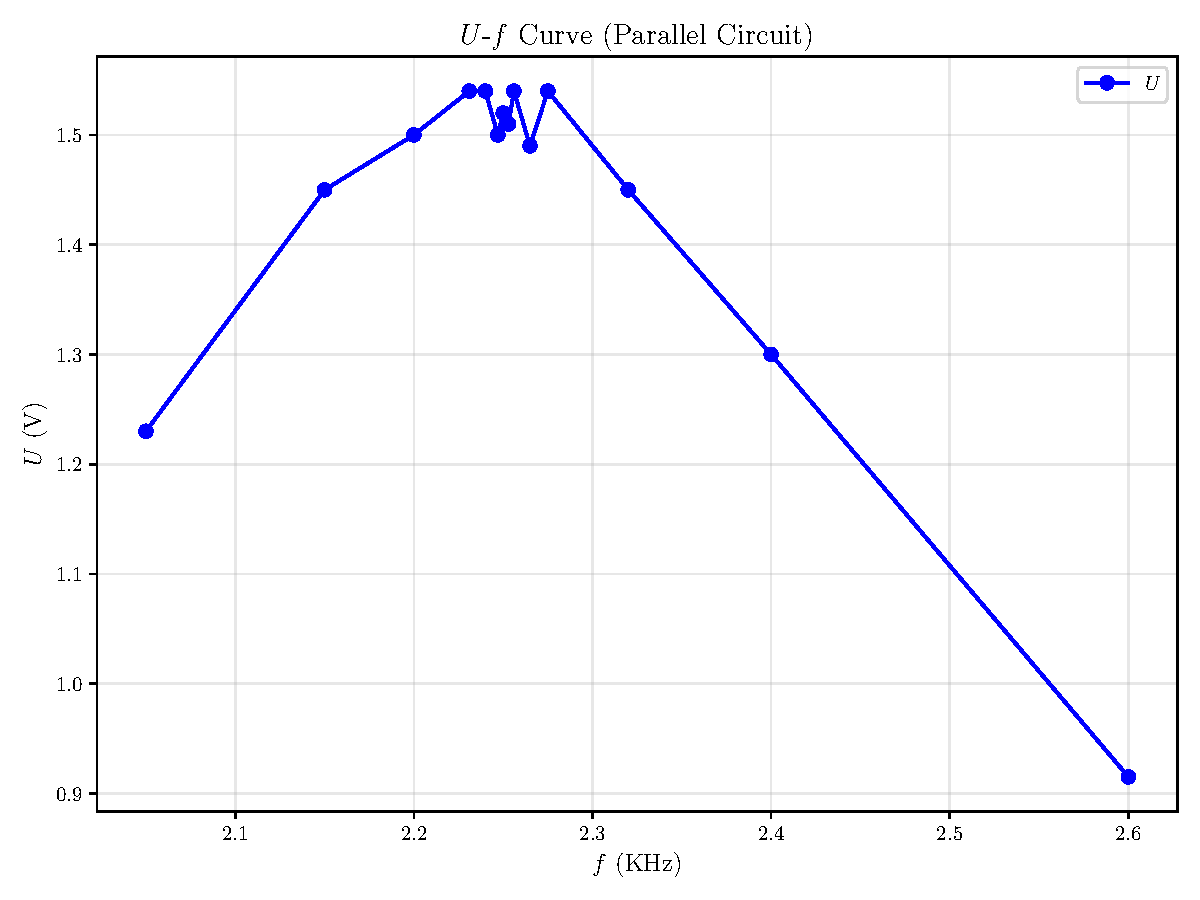
\includegraphics[width=0.8\textwidth]{./parallel_circuit_u_f.pdf}
    \caption{RLC并联电路$u - f$曲线}
    \label{fig:parallel_circuit_u_f}
\end{figure}

\begin{figure}[H]
    \centering
    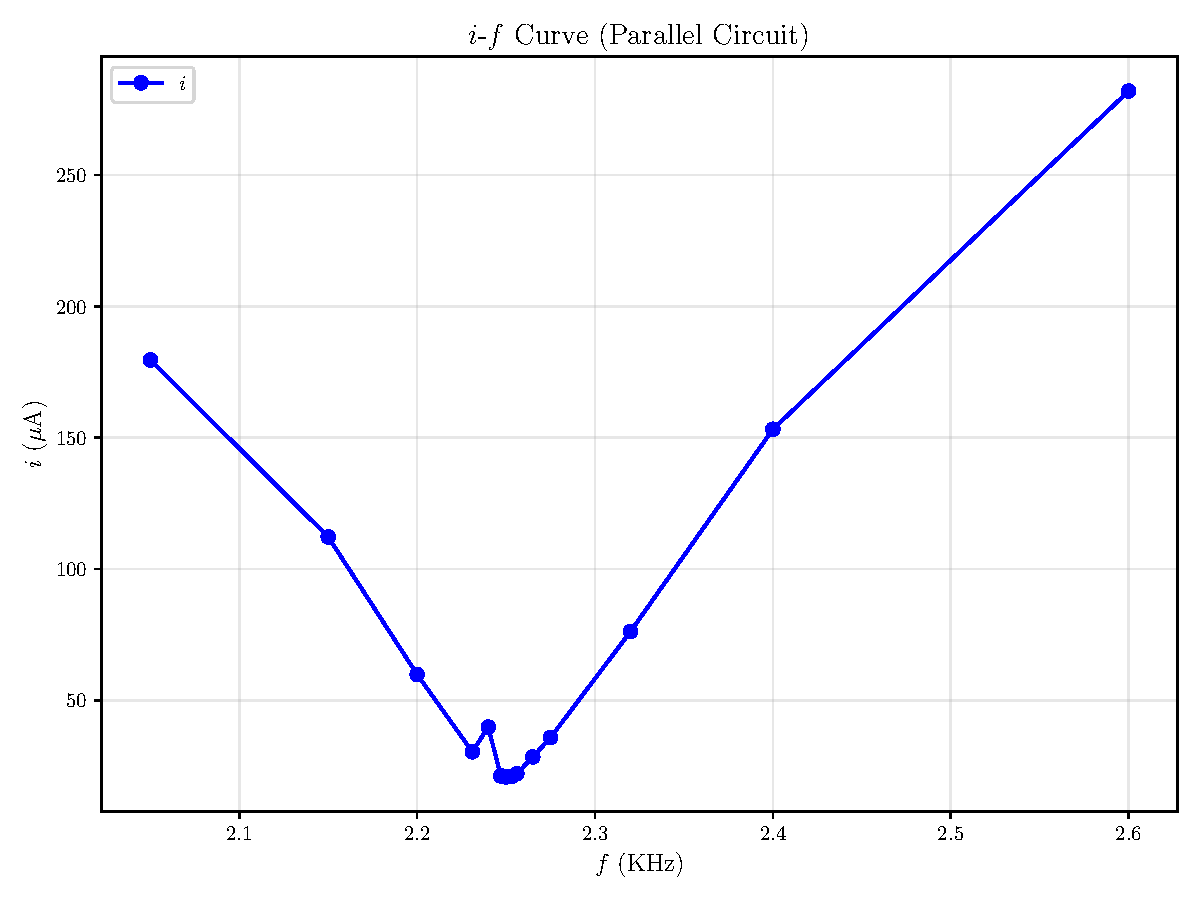
\includegraphics[width=0.8\textwidth]{./parallel_circuit_i_f.pdf}
    \caption{RLC并联电路$i - f$曲线}
    \label{fig:parallel_circuit_i_f}
\end{figure}

\subsection{观测RLC串联电路的暂态过程}

由函数发生器产生方波，函数发生器各参数可设为：频率50 Hz，电压峰峰值=2.0 V，偏移1V。示波器CH1通道用来测量总电压，CH2用来测量电容两端电压，注意两个通道必须共地。
\begin{enumerate}
    \item \( R = 0 \, \Omega \)，测量 \( u_C \) 波形如图：

      \begin{figure}[H]
        \centering
        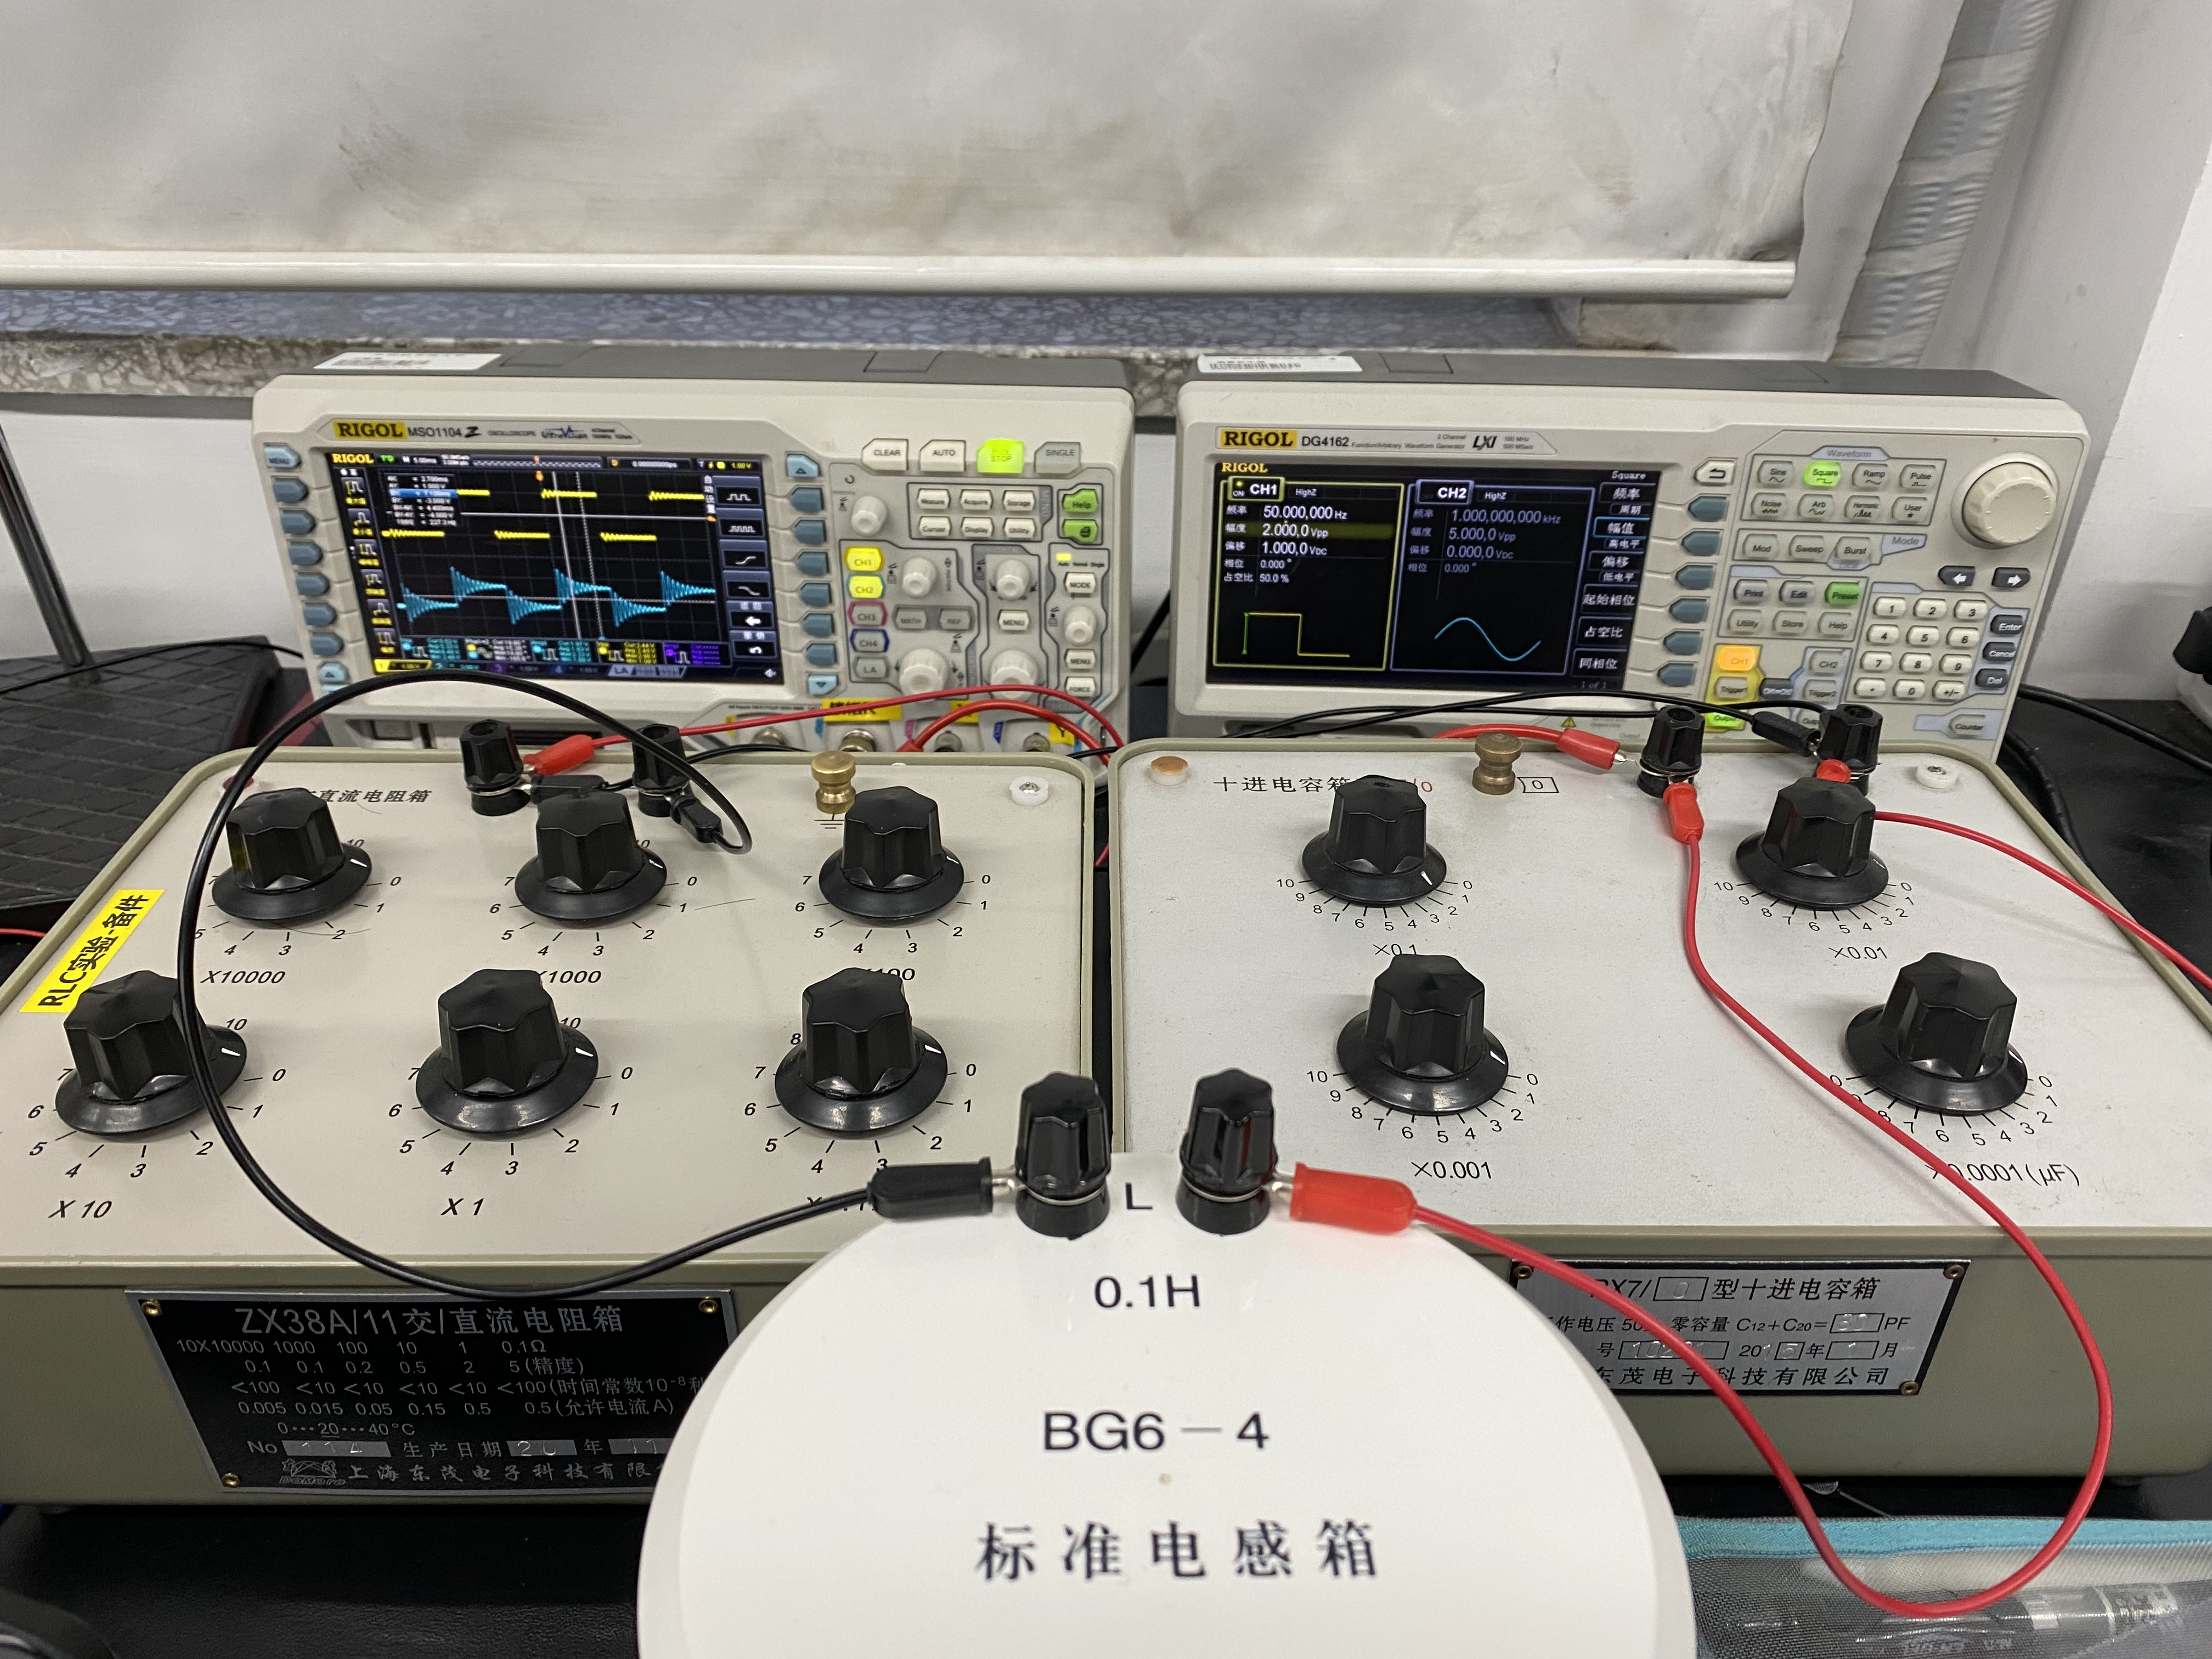
\includegraphics[width=0.8\textwidth]{./transient_process_R_0.jpg}
        \caption{RLC串联电路的暂态过程，\( R = 0 \, \Omega \)}
        \label{fig:transient_process_R_0}
      \end{figure}

    \item 调节 \( R \) 测得临界电阻 \( R_C \)，并与理论值比较。

      \begin{figure}[H]
        \centering
        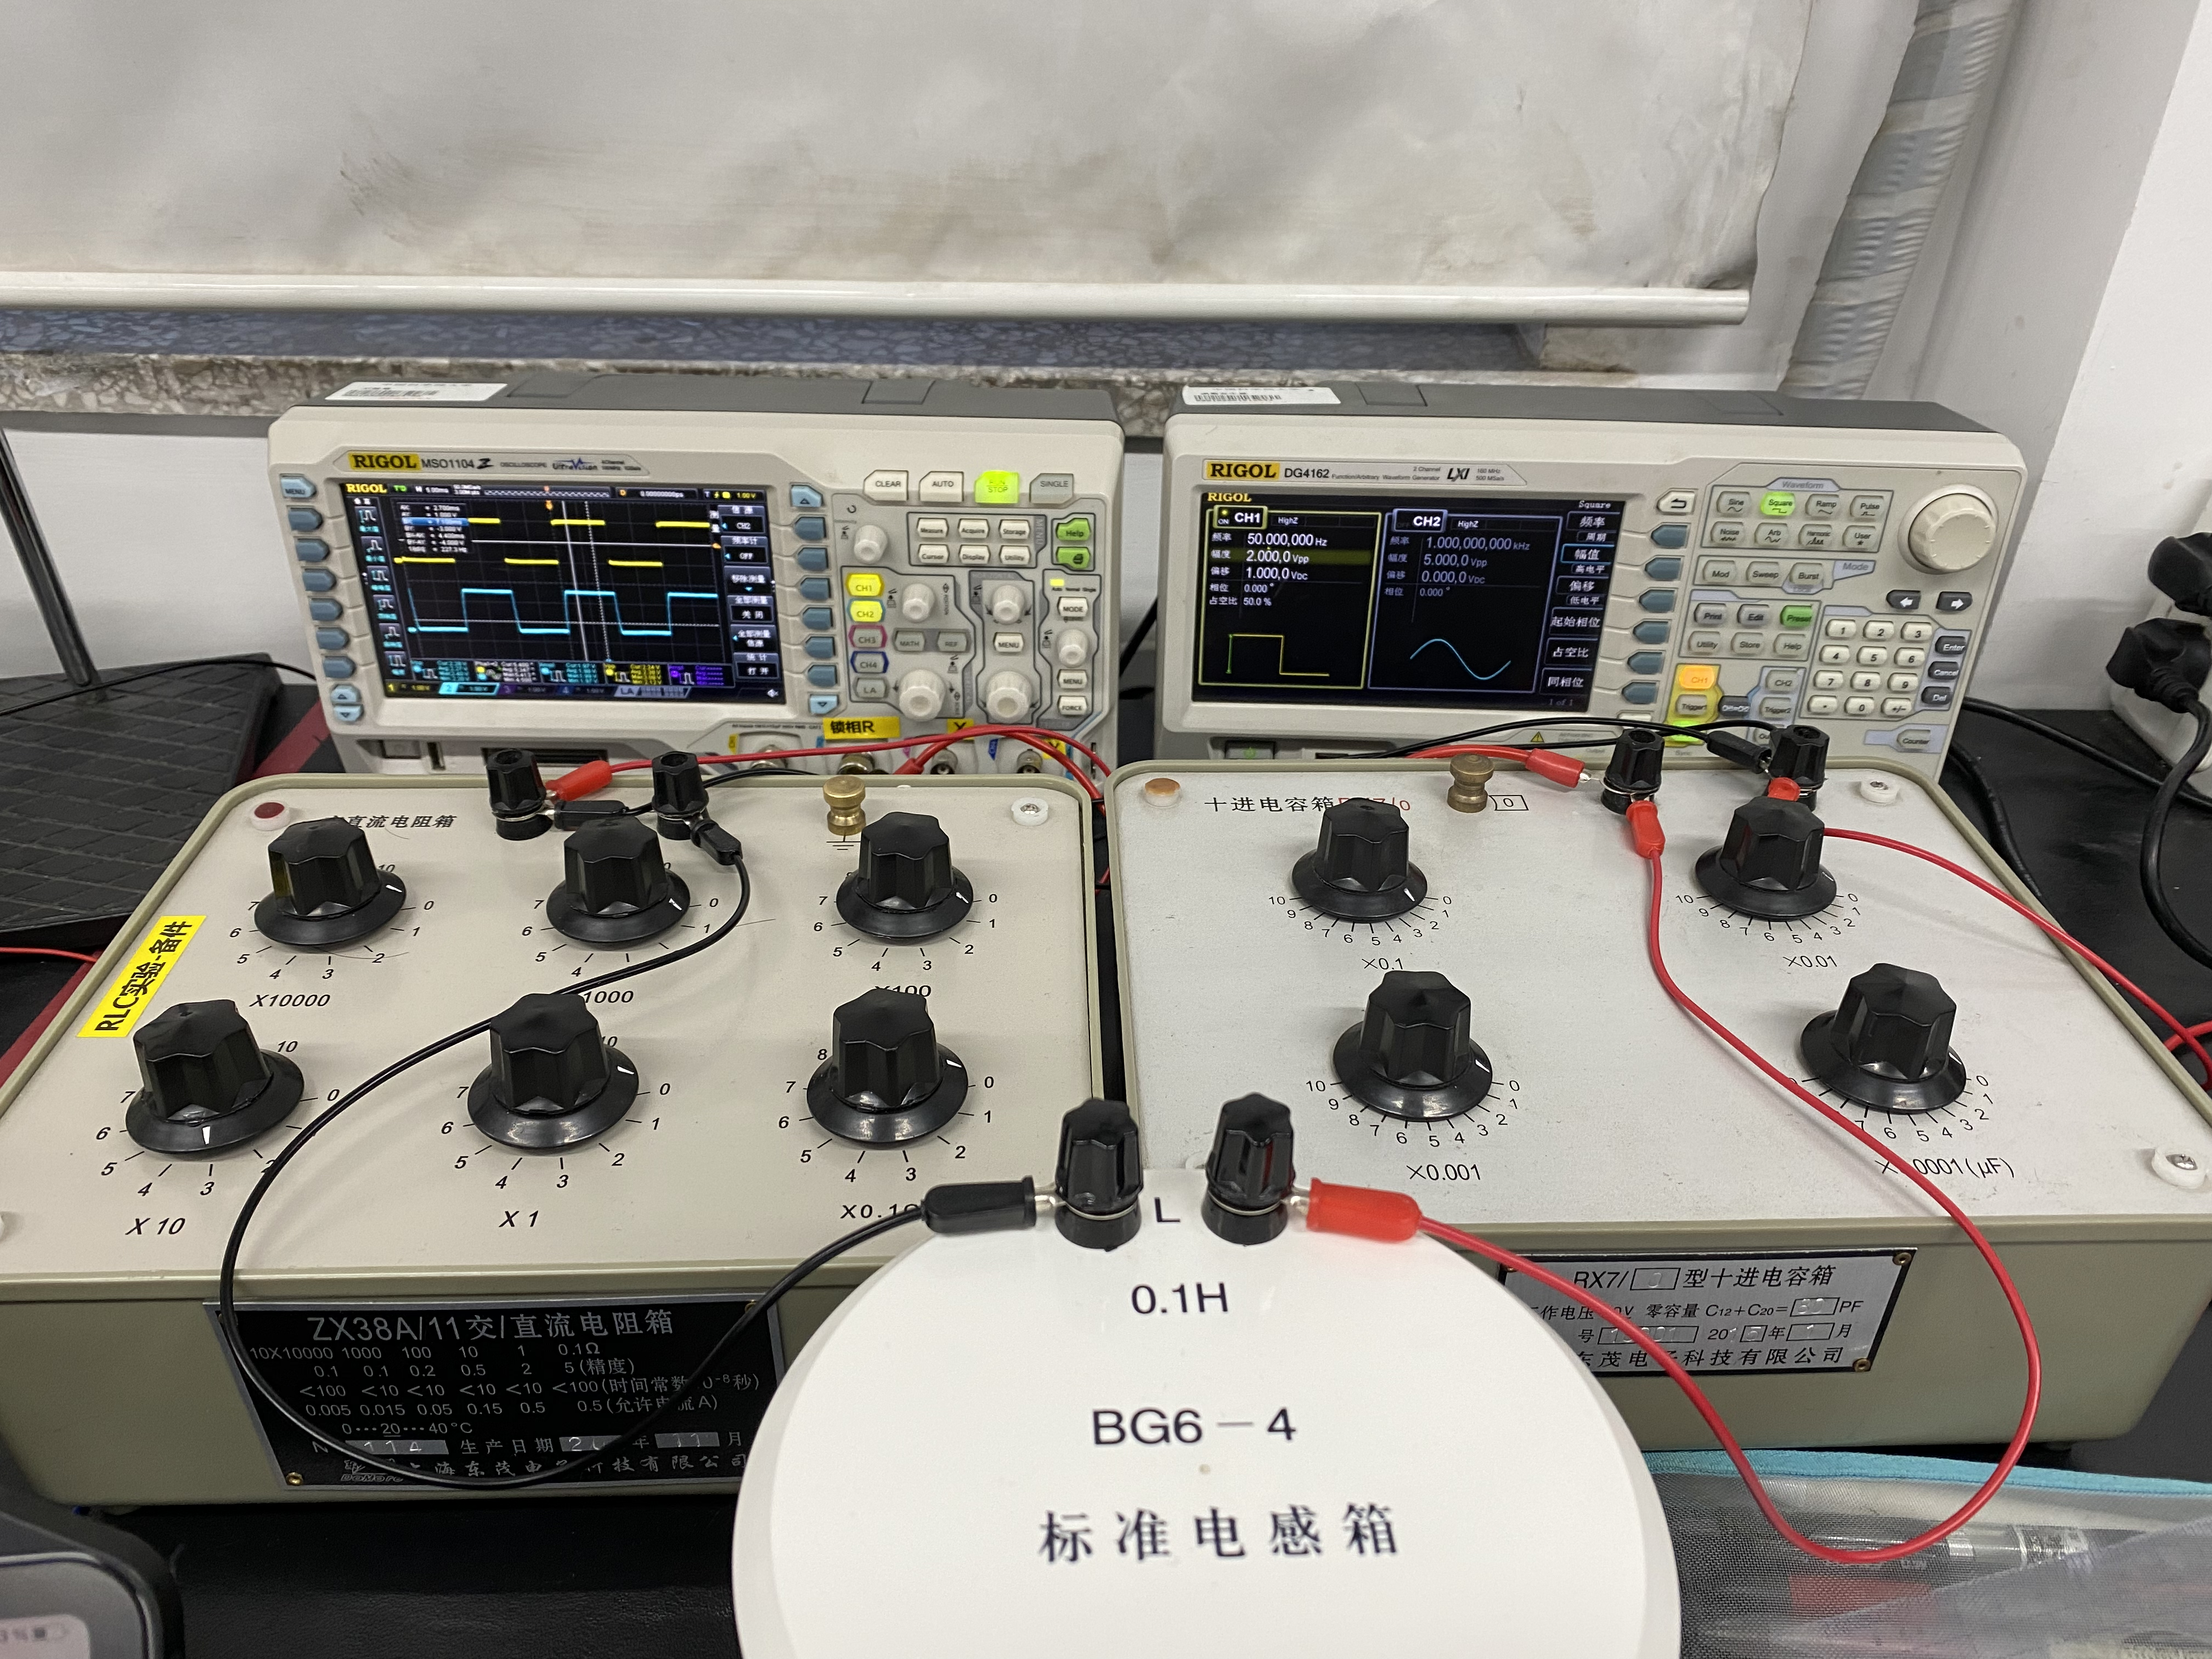
\includegraphics[width=0.8\textwidth]{./critical_resistance}
        \caption{临界电阻}
        \label{fig:critical_resistance}
      \end{figure}

      根据公式 $R^2 = \$ frac{4L}{C}$ 计算出临界电阻 $R_C = 1.414 \, \text{k}\Omega$，根据图 \ref{fig:critical_resistance} 可知，临界电阻 \( R_C \) 约为 1.130 k$\Omega$，与理论值相比，误差约为 20.2\%。出现这一结果的原因可能是因为电感存在一定的电阻，这一电阻未被考虑。也可能是因为，电容与电感的实际值与标定的值存在偏差。此外，示波器上调节电阻后波形的变化比较细微，因此难以掌握到达临界电阻的确切位置。

    \item 记录 \( R = 2 \, \text{k}\Omega \)，\( 20 \, \text{k}\Omega \) 的 \( u_C \) 波形。函数发生器频率可分别选为 250 Hz（\( R = 2 \, \text{k}\Omega \)），和 20 Hz（\( R = 20 \, \text{k}\Omega \)），示波器上的波形如下：
    
    \begin{figure}[h]
    \centering
    % 第一张图
    \begin{subfigure}[b]{0.45\textwidth}
        \centering
        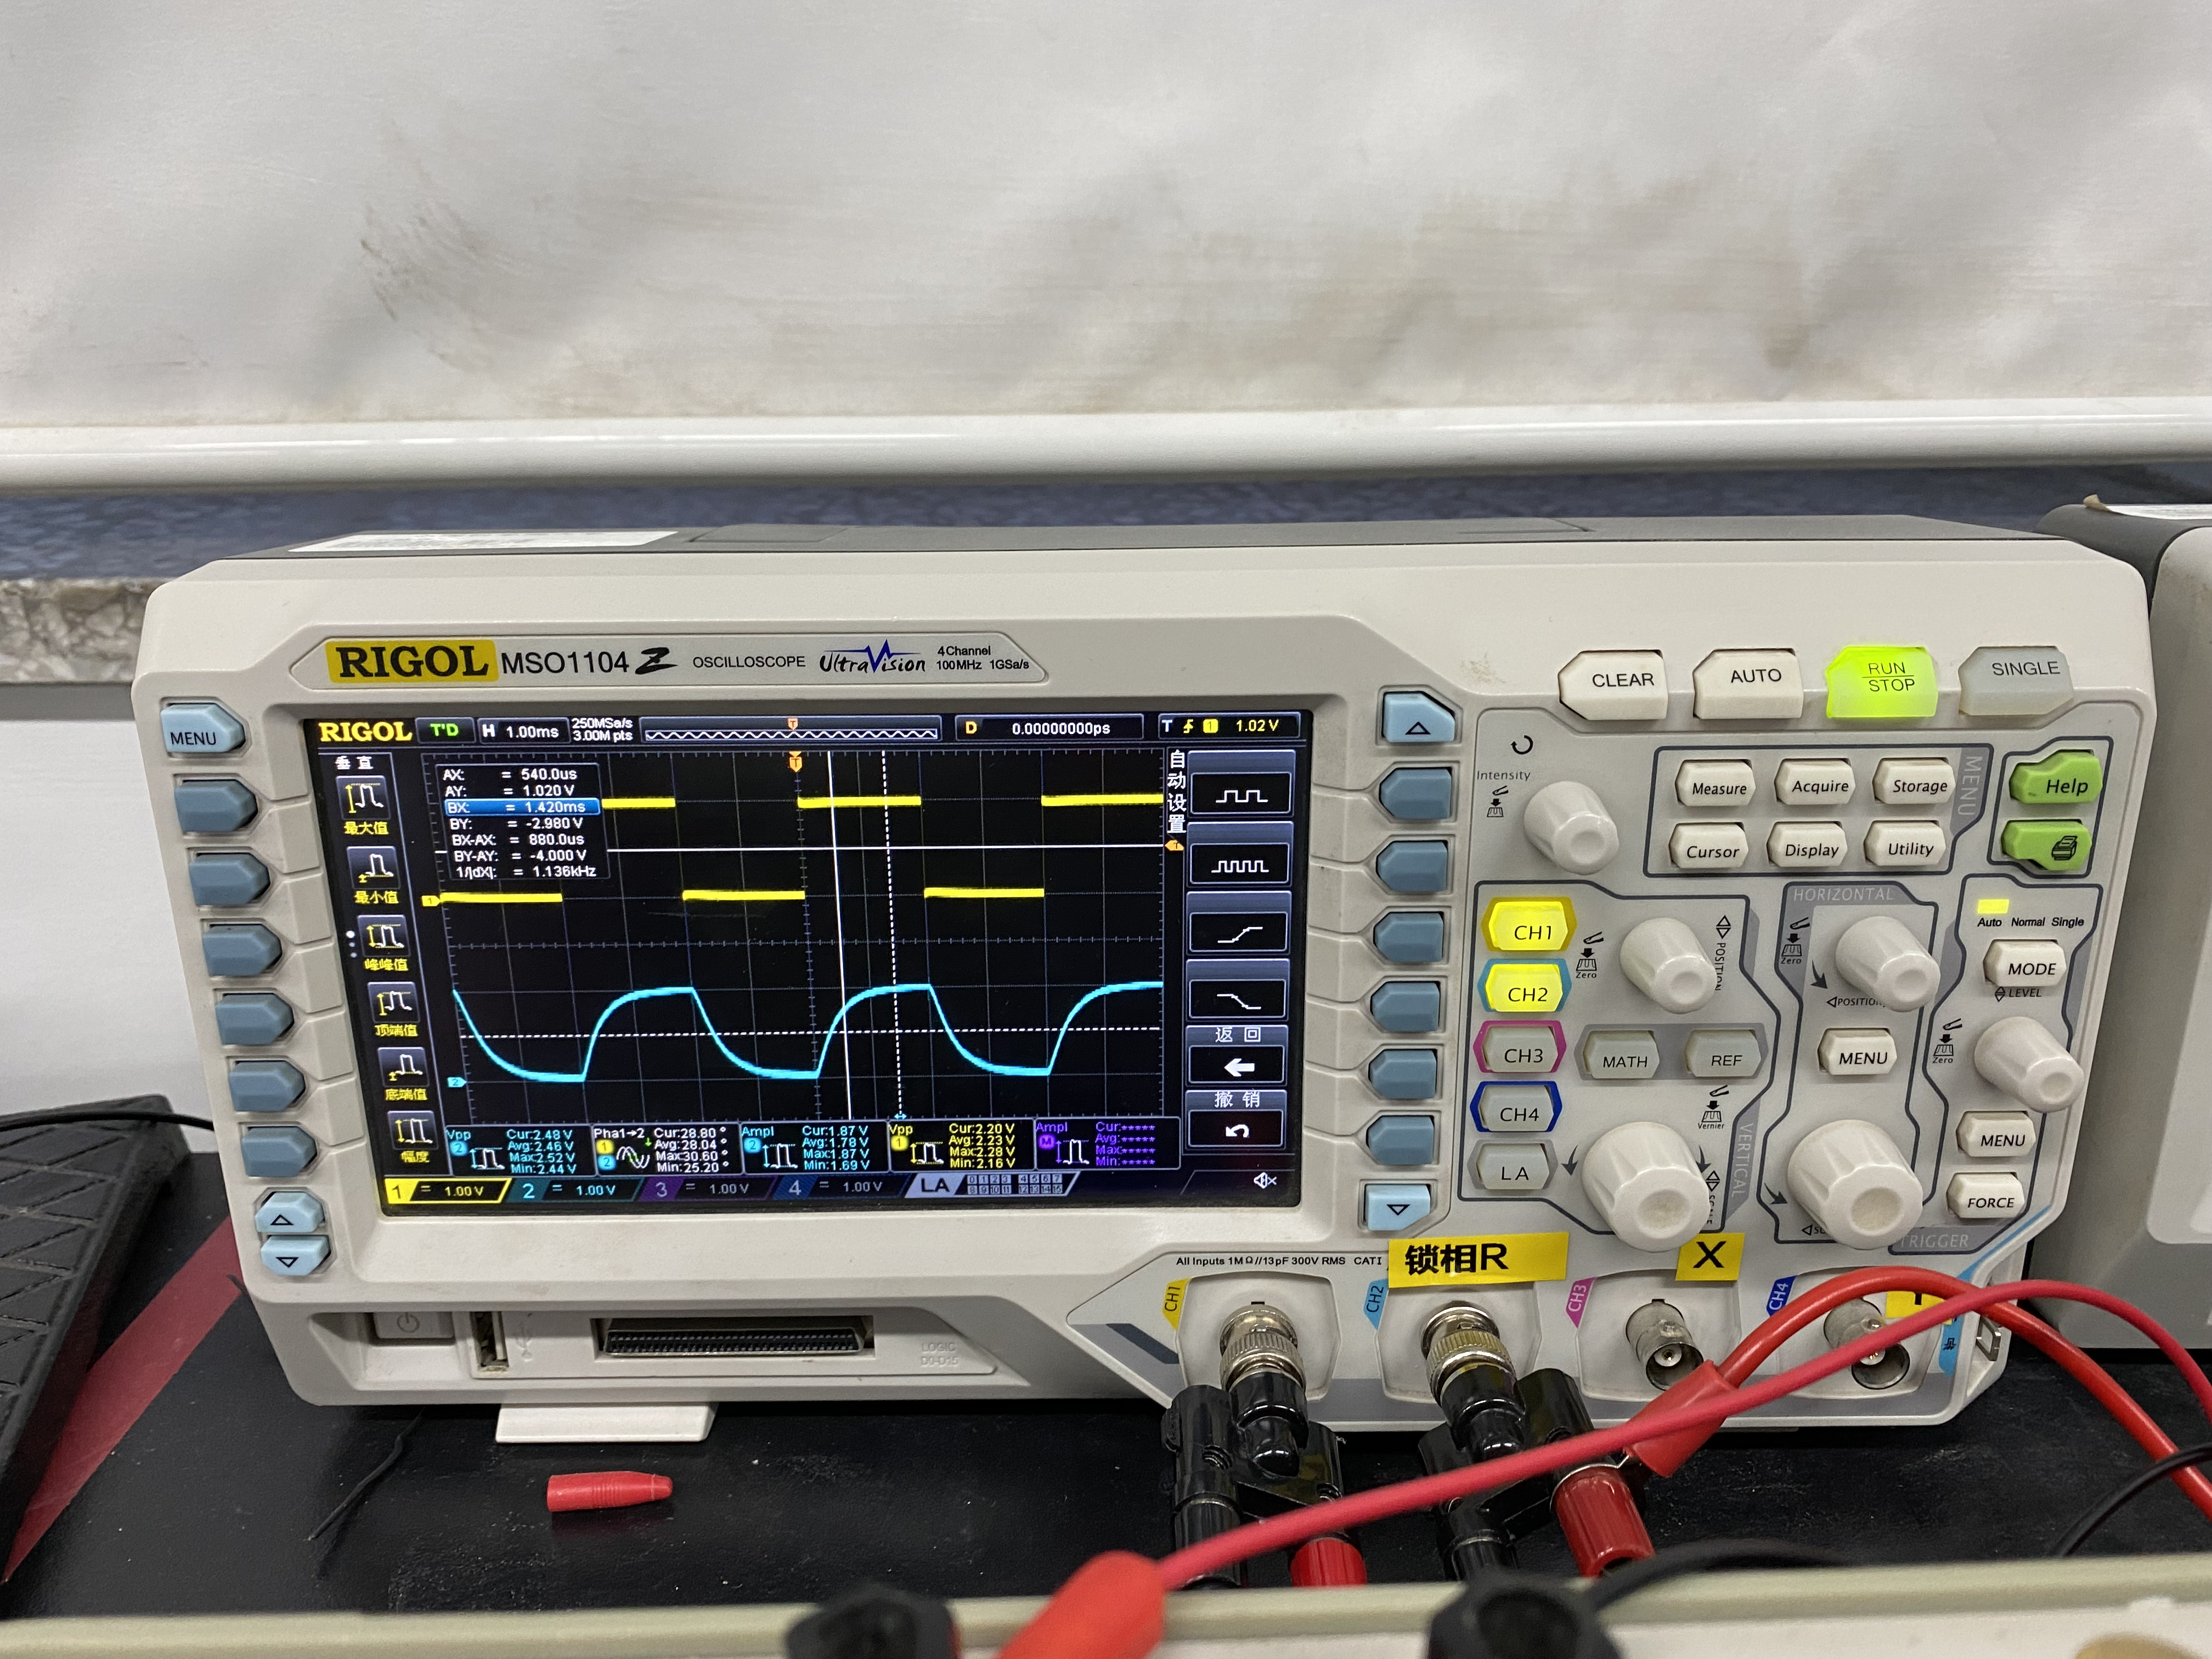
\includegraphics[width=\textwidth]{./250hz_wave.jpg}
        \caption{\( f = 250 \, \text{Hz} \)时的波形}
        \label{fig:250hz_wave}
    \end{subfigure}
    \hfill
    % 第二张图
    \begin{subfigure}[b]{0.45\textwidth}
        \centering
        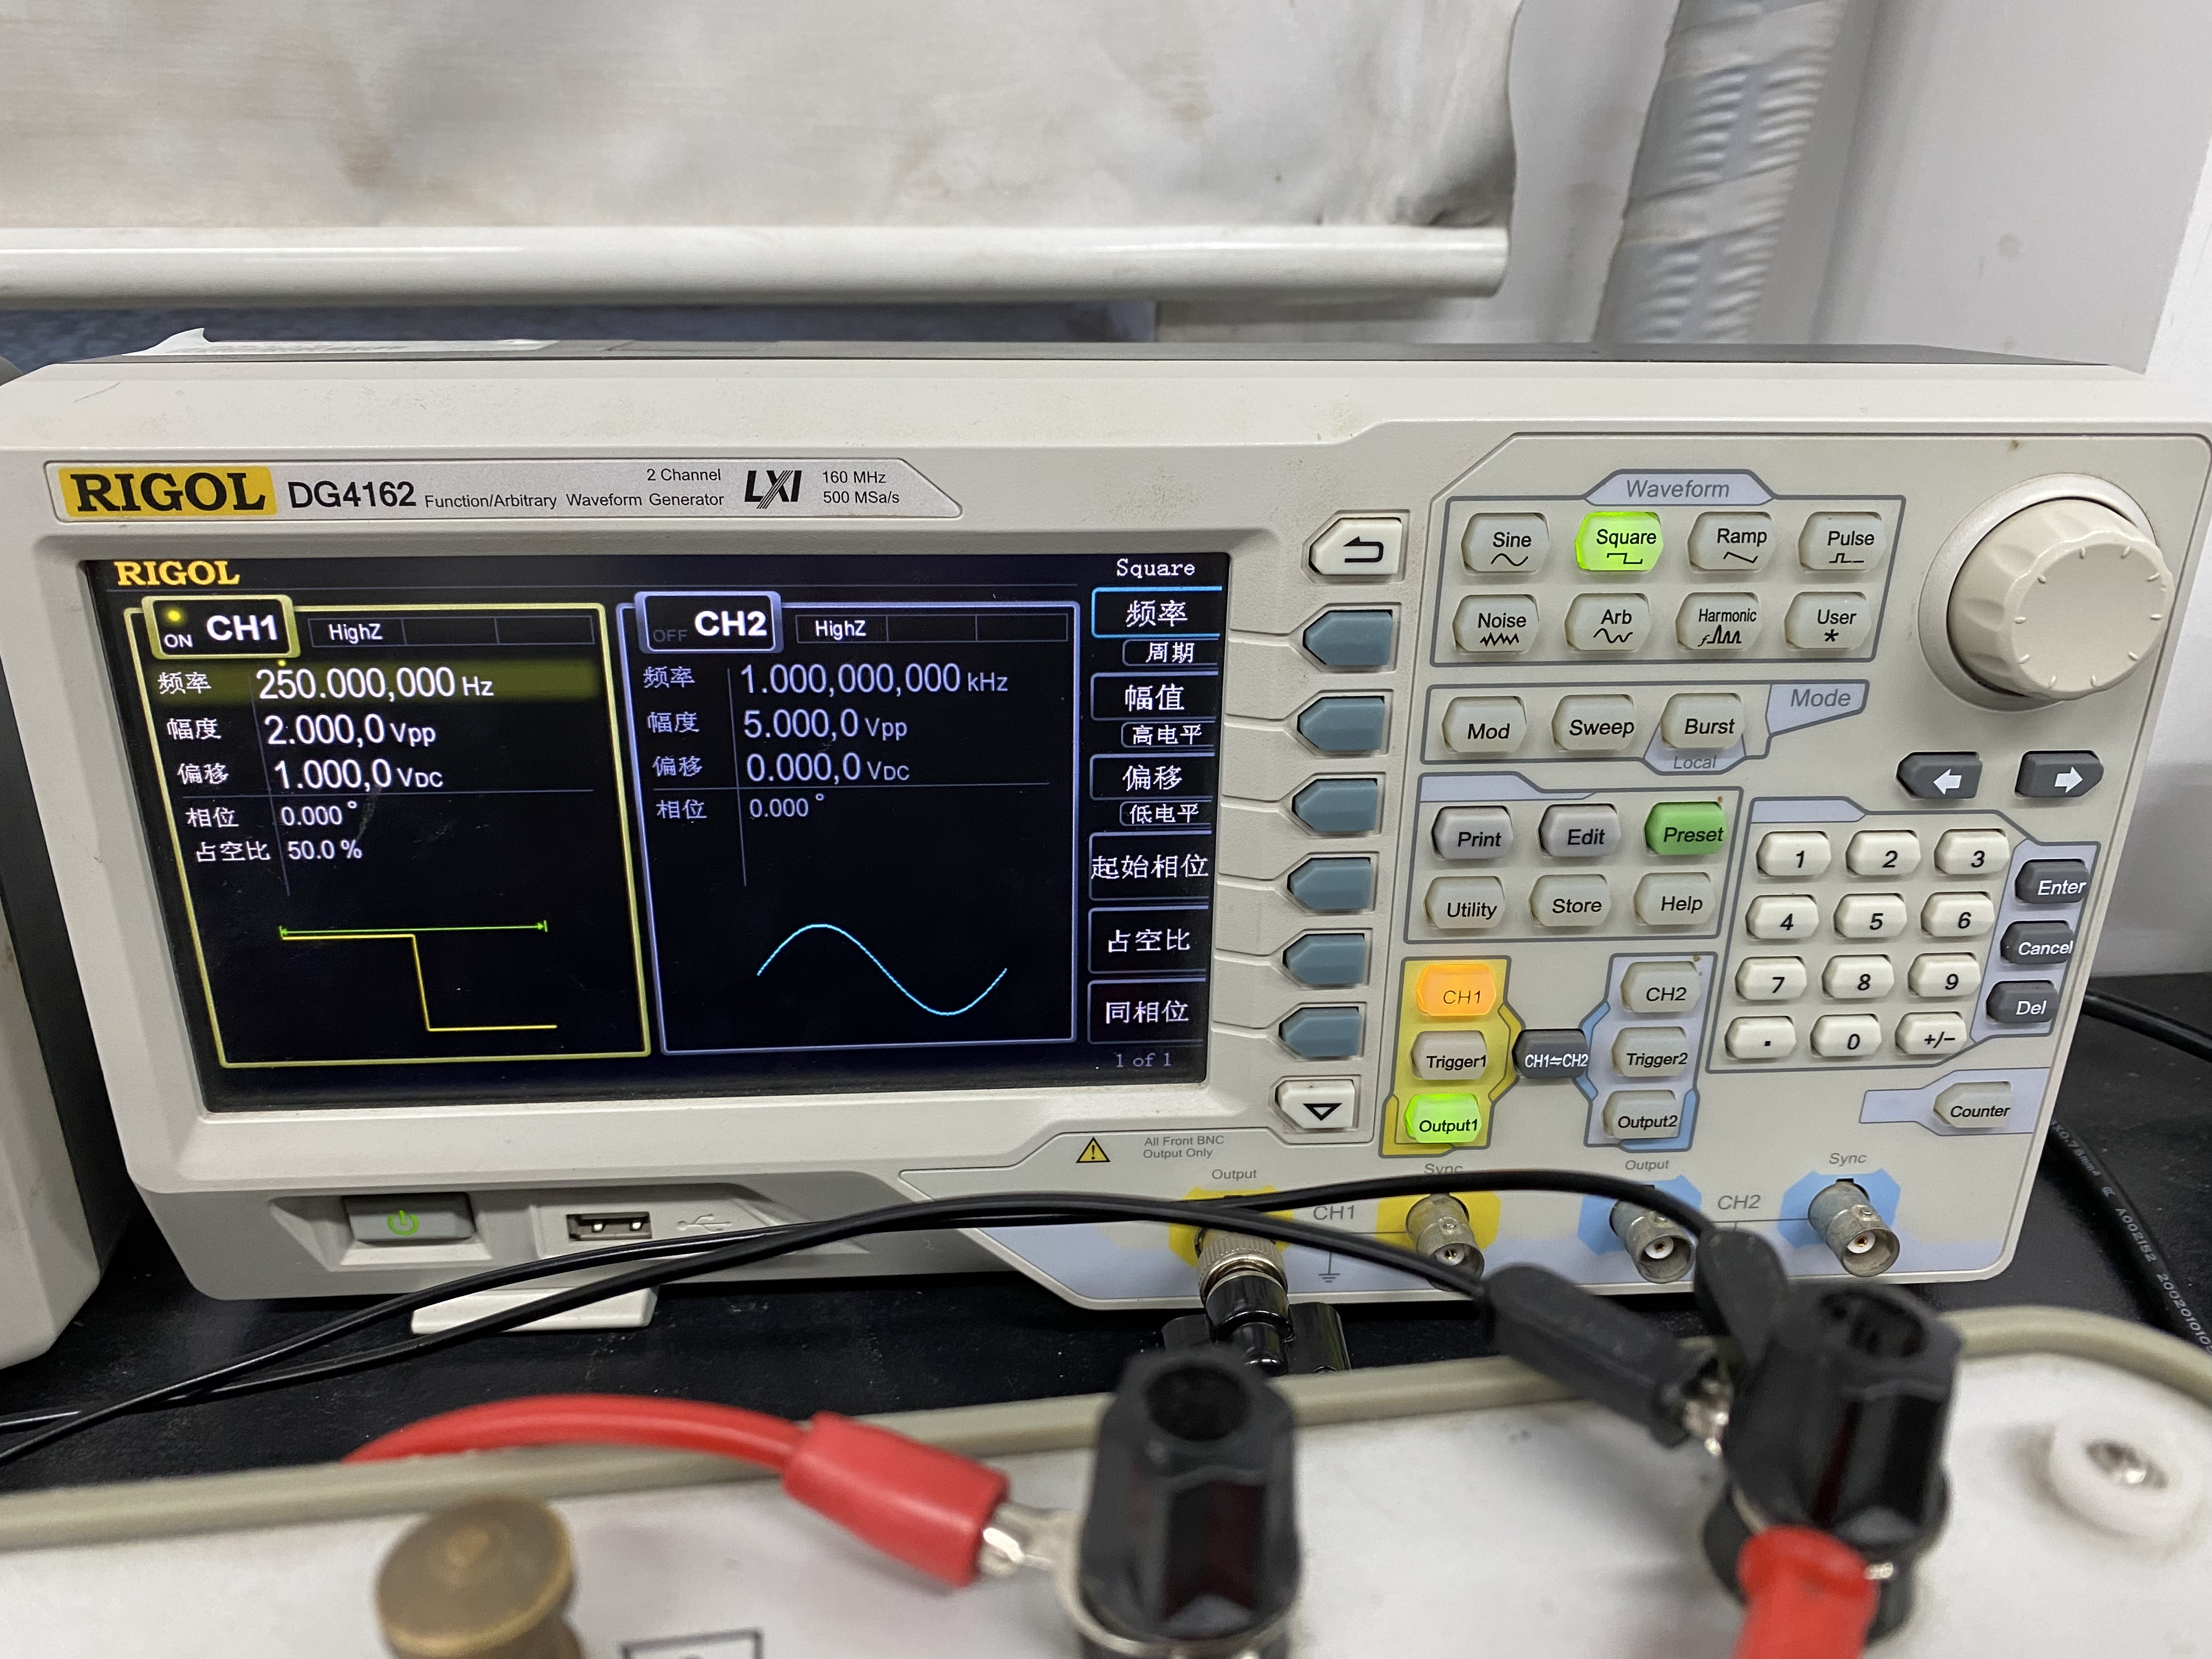
\includegraphics[width=\textwidth]{./250hz_signal.jpg}
        \caption{\( f = 250 \, \text{Hz} \)时的信号发生器界面}
        \label{fig:250hz_signal}
    \end{subfigure}

    \caption{频率为 250 Hz 时的波形和信号发生器界面}
    \label{fig:parallel-circuits}
\end{figure}

    \begin{figure}[h]
    \centering
    % 第一张图
    \begin{subfigure}[b]{0.45\textwidth}
        \centering
        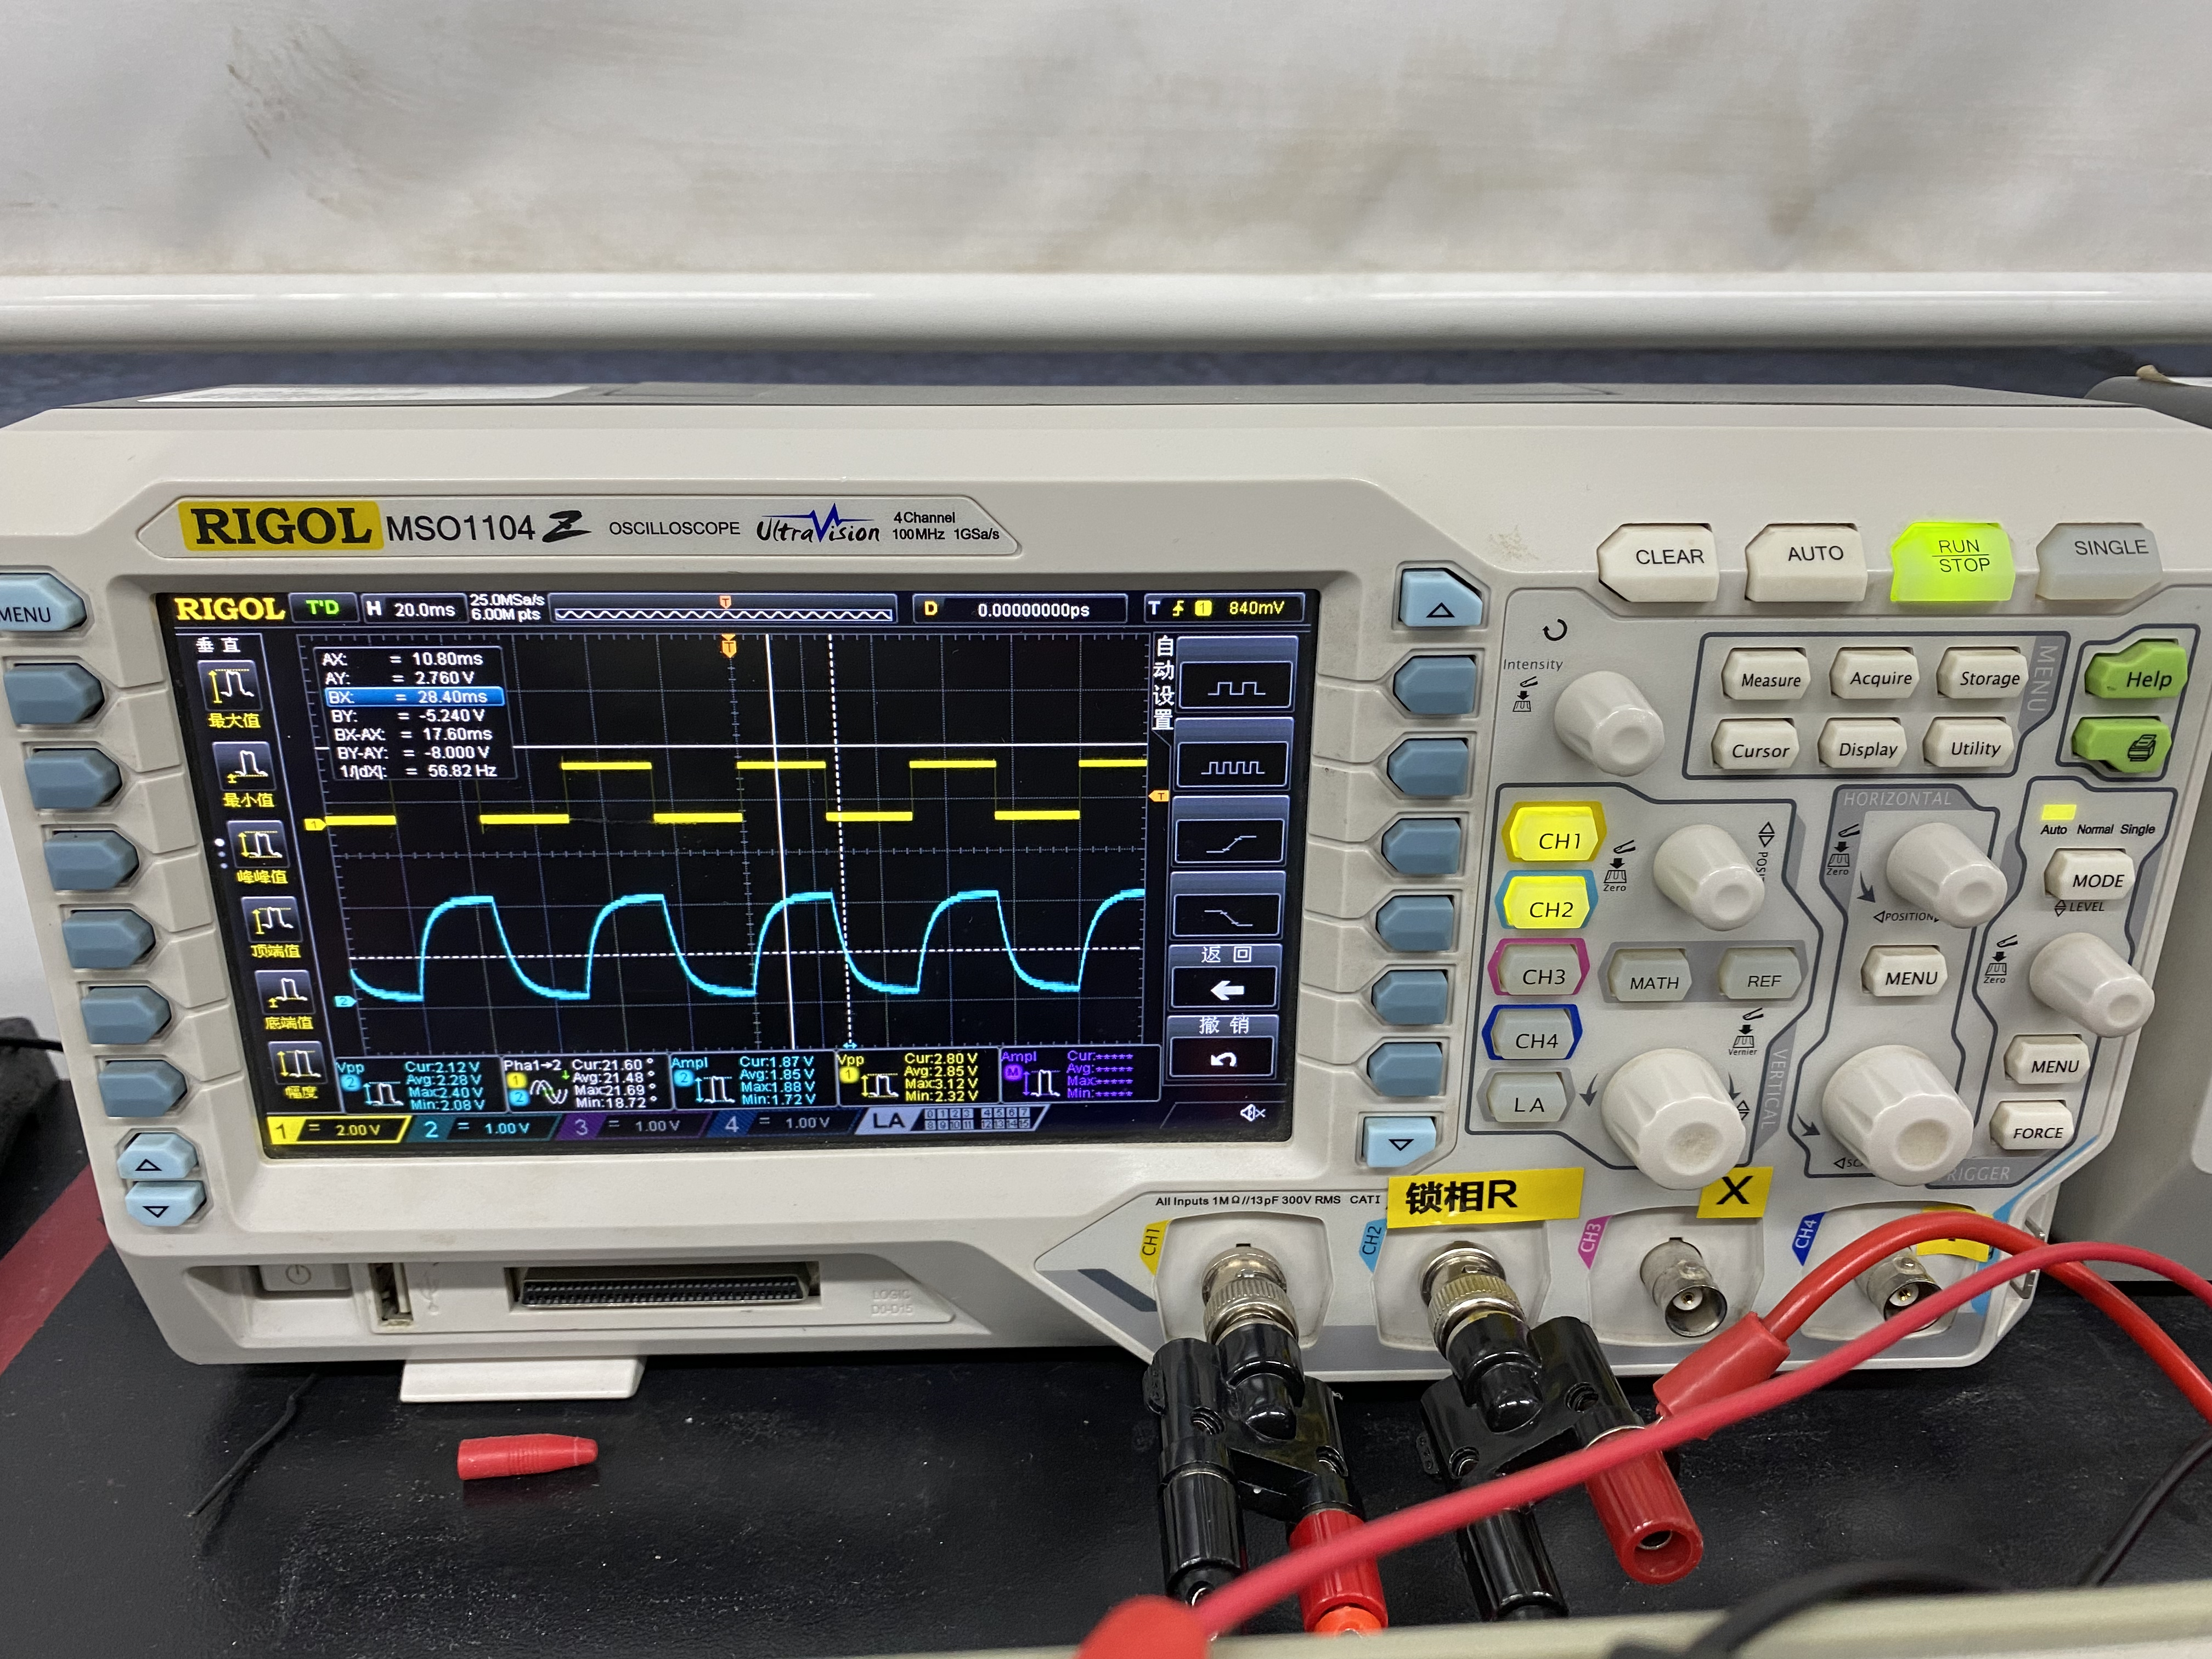
\includegraphics[width=\textwidth]{./20hz_wave.jpg}
        \caption{\( f = 20 \, \text{Hz} \)时的波形}
        \label{fig:20hz_wave}
    \end{subfigure}
    \hfill
    % 第二张图
    \begin{subfigure}[b]{0.45\textwidth}
        \centering
        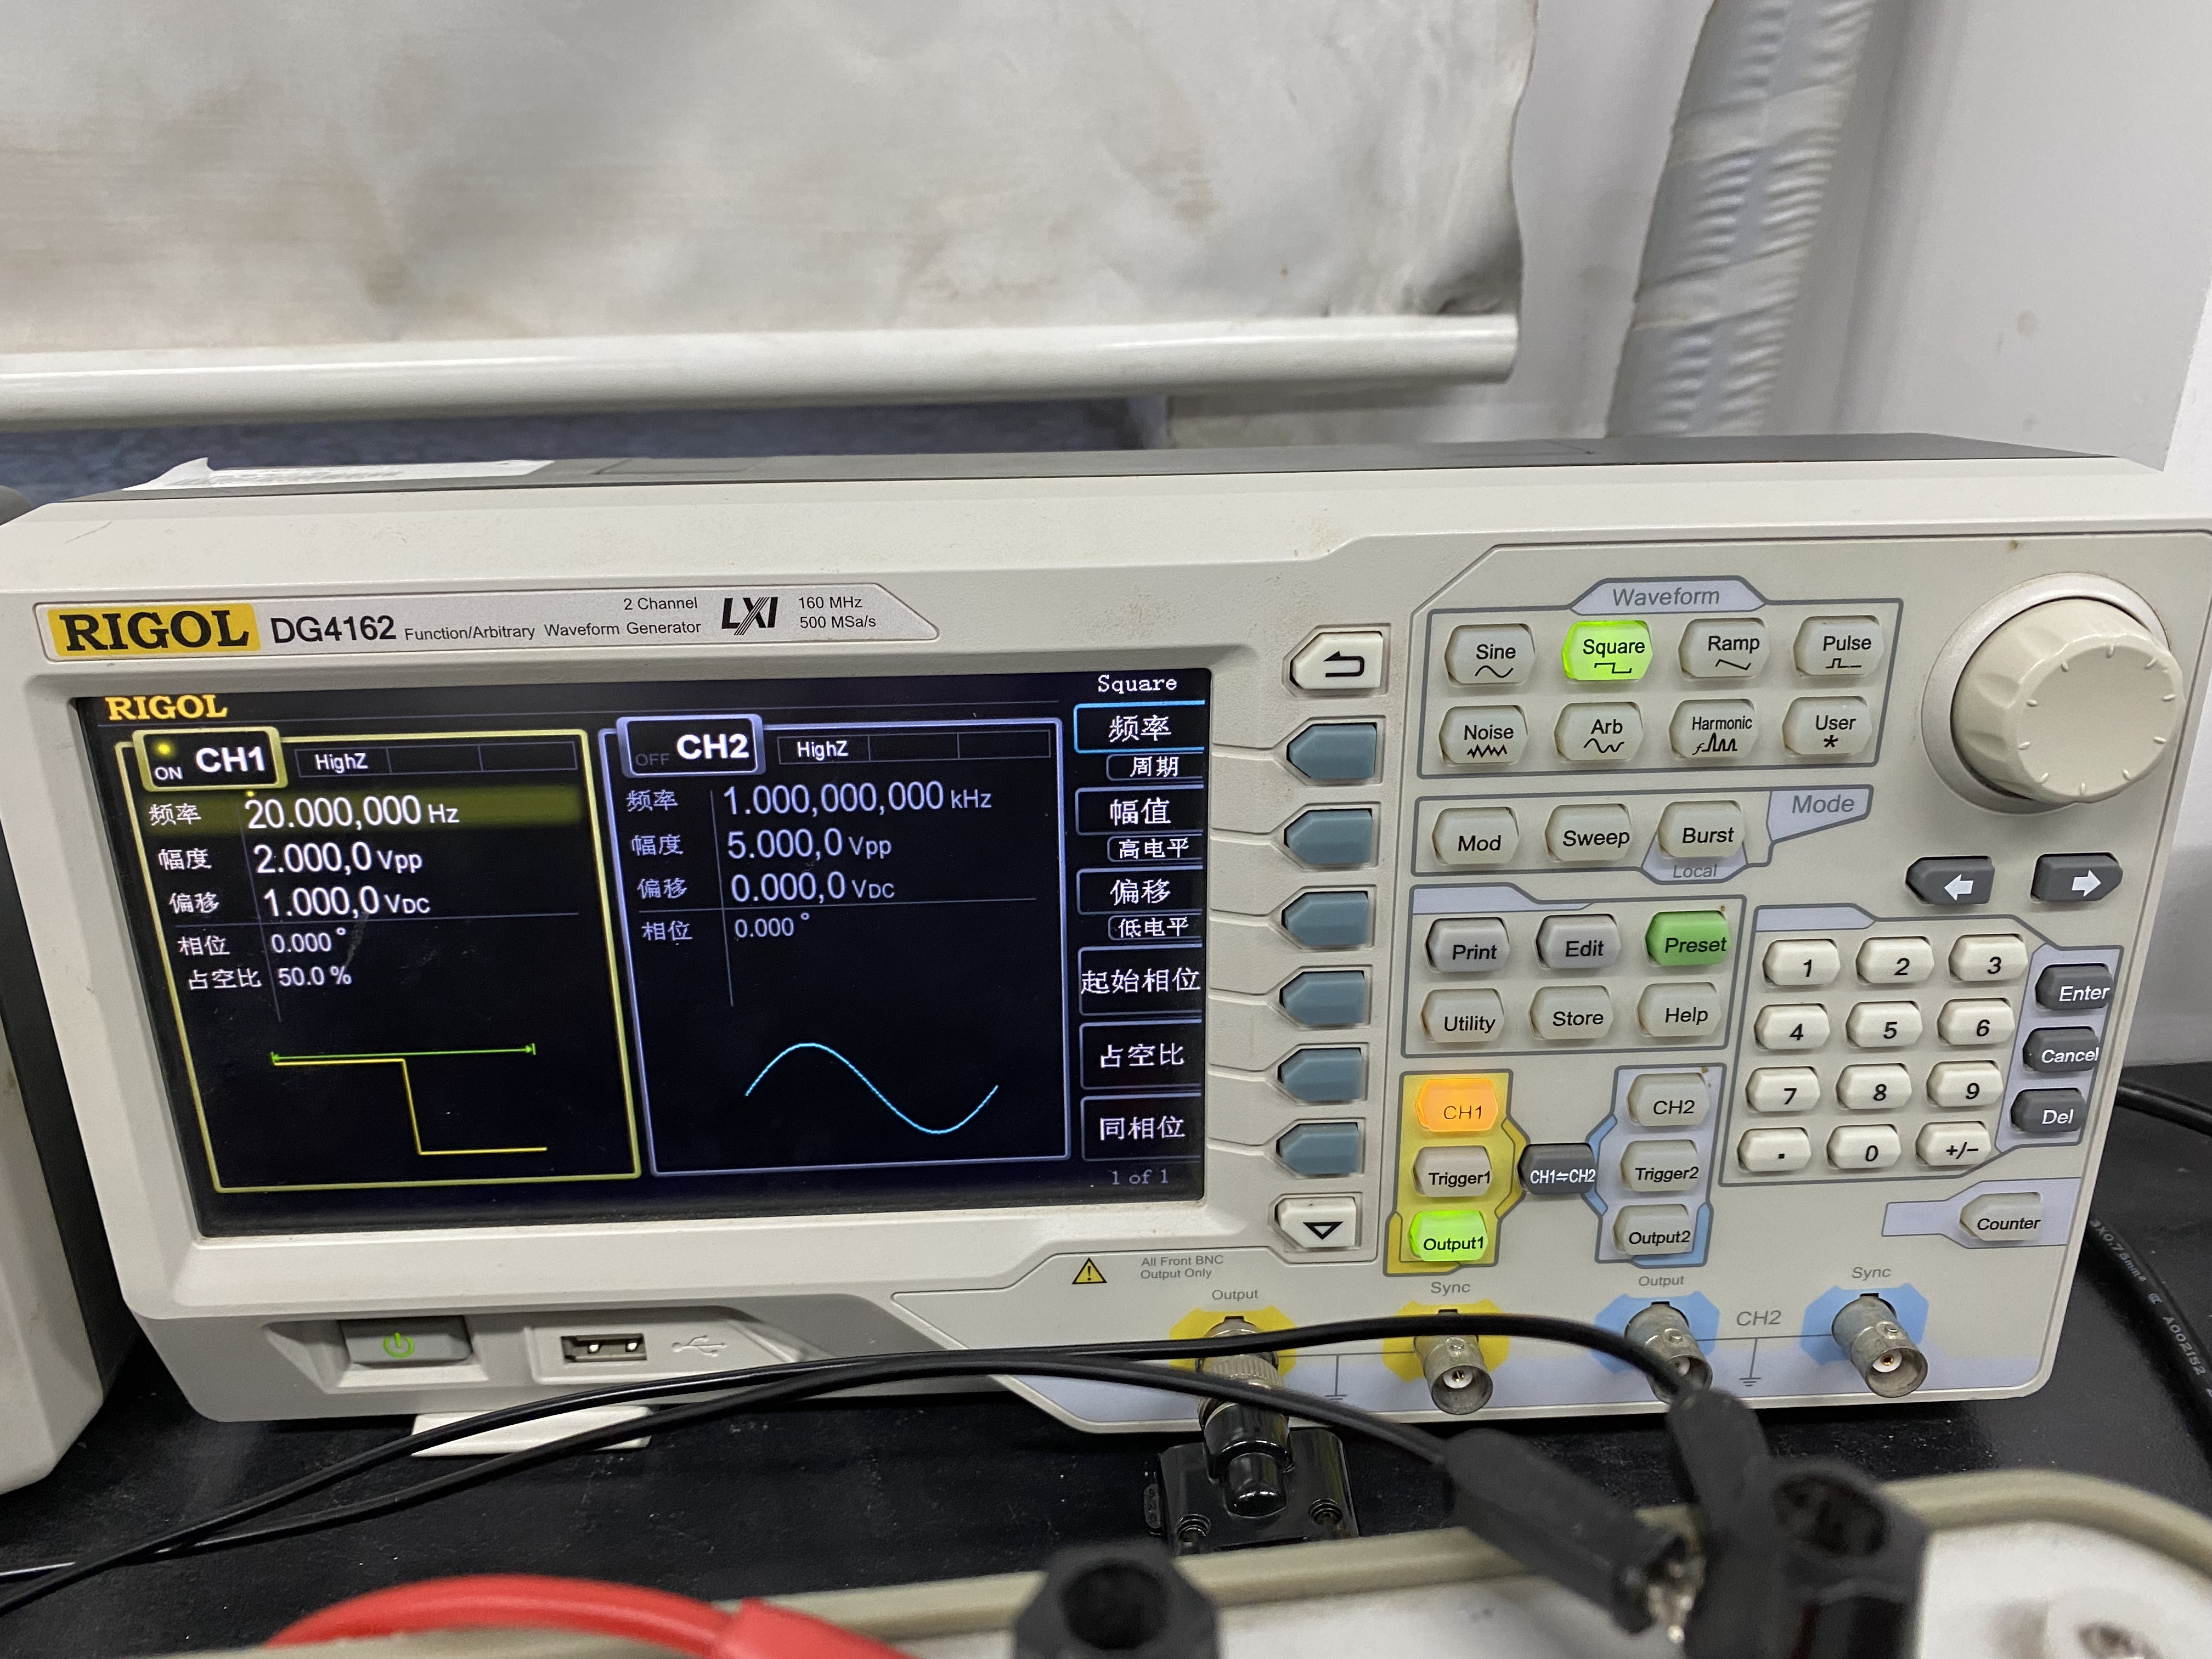
\includegraphics[width=\textwidth]{./20hz_signal.jpg}
        \caption{\( f = 20 \, \text{Hz} \)时的信号发生器界面}
        \label{fig:20hz_signal}
    \end{subfigure}

    \caption{频率为 20 Hz 时的波形和信号发生器界面}
    \label{fig:parallel-circuits}
\end{figure}

\end{enumerate}

\section{思考与讨论}

\begin{itemize}
  \item 在测量 RLC 串联电路和并联电路的相频特征和幅频特征曲线的过程中，探头要从示波器的默认值 $10 \times$ 调整到 $1 \times$，否则示波器显示的电压幅值并不是真正的幅值，将会导致非常大的误差。
  \item 为了使测量的参数更加稳定，本实验在测量的过程中需要使用示波器的统计功能，但在改变频率测量下一个数值之前需要关闭并重新开启统计功能，否则，下一个实验数据的测量会受到上一个数值的影响。
  \item 在测量 RLC 并联电路的相频特性和幅频特性曲线的过程中，需要使用示波器的光标功能来读取相同相位点的时间间隔 $\Delta t$ 。此时最好在每一次测量时都用实线光标对准一个信号，而虚线光标对准另一个。保持这种对应关系不变会减少符号处理上的问题。
  \item 在调节频率时每一次都需要检查串并联电路的路端电压是否为 2.0V，如果不是，需要调节函数发生器的输出电压，以保证测量的准确性。
  \item 在实验过程中，必须特别注意确保设备共地。以串联谐振实验为例，若示波器未能共地，例如 CH1 的地端连接在 a 点，CH2 的地端连接在 b 点，则 a 和 b 点同时接地，电压为 0。这种情况下，电感、电容和电阻三种元件上都不会有电流通过，电路被短路，实验无法进行。其他未共地的情况也会导致类似结果：电路中的某些元件处于两个接地点之间，且没有电源提供电压，因而会被短路。
\end{itemize}

\section{参考资料}
本实验报告有适当参考讲义及圣遗物。

\section{原始数据记录表}
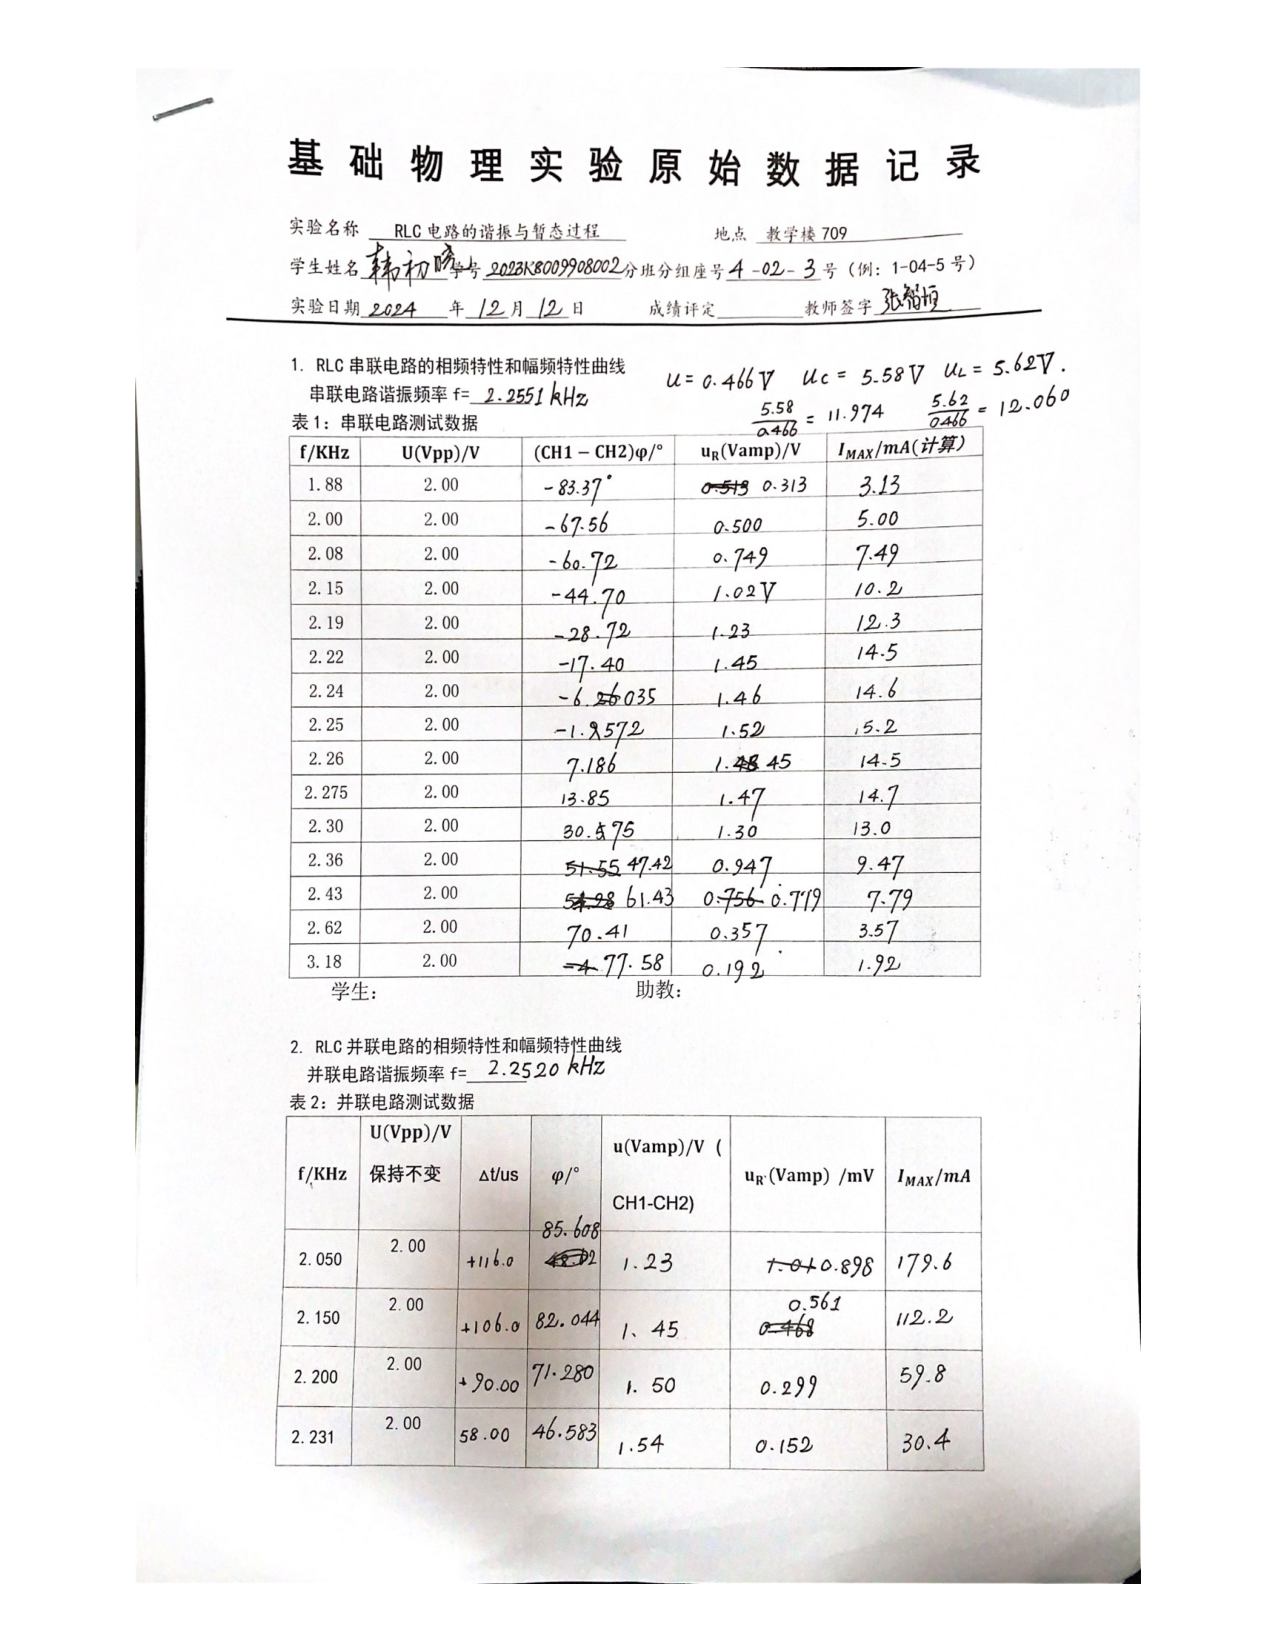
\includepdf[pages=-]{./韩初晓- RLC谐振电路-数据.pdf}

\end{document}

% VScode 常用快捷键：

% F2:                       变量重命名
% Ctrl + Enter:             行中换行
% Alt + up/down:            上下移行
% 鼠标中键 + 移动:           快速多光标
% Shift + Alt + up/down:    上下复制
% Ctrl + left/right:        左右跳单词
% Ctrl + Backspace/Delete:  左右删单词    
% Shift + Delete:           删除此行
% Ctrl + J:                 打开 VScode 下栏(输出栏)
% Ctrl + B:                 打开 VScode 左栏(目录栏)
% Ctrl + `:                 打开 VScode 终端栏
% Ctrl + 0:                 定位文件
% Ctrl + Tab:               切换已打开的文件(切标签)
% Ctrl + Shift + P:         打开全局命令(设置)

% Latex 常用快捷键：

% Ctrl + Alt + J:           由代码定位到PDF


